\chapterimage{chapter_head_musicos1.pdf} % Chapter heading image

\chapter{Fundamentos de composição musical}
\label{cap:musicacomposer}
Nas seguintes sub seções abordaremos alguns conceitos importantes para iniciar o estudo da composição musical;
porem, não aprofundaremos demasiado em toda a teoria, 
devido a que as explicações mostradas aqui, estão
orientadas para um público interessado na dança, que necesita a principio
ferramentas para entender a música e pode depois melhorar sua percepção musical. 


%%%%%%%%%%%%%%%%%%%%%%%%%%%%%%%%%%%%%%%%%%%%%%%%%%%%%%%%%%%%%%%%%%%%%%%%%%%%%%%%
\section{Consonância e dissonância}
\index{Música!Consonância}
\label{sec:consonancia}

\begin{tcbinformation} 
\index{Música!Consonância}
\label{ref:consonancia}
\textbf{Consonância (Música):}
Relação de tons soando agradáveis e estáveis ao ouvido \cite[pp. 26]{wright2012essential}.
Algumas combinações de teclas no piano produzem um som agradável e harmonioso.
\end{tcbinformation} 


\begin{tcbinformation} 
\index{Música!Dissonância}
\label{ref:dissonancia}
\textbf{Dissonância (Música):}
Relação de tons soando desagradáveis e instáveis ao ouvido \cite[pp. 26]{wright2012essential}.
Algumas combinações de teclas no piano produzem um som áspero e estridente.
\end{tcbinformation} 



A escola Pitagórica, que existiu no seculo VI (A.C.),
tentava compreender o universo;
com esse fim desenharam modelos matemáticos para explicar 
os fenômenos observados.
Entre os temas que foram tratados estava incluída a música,
e porquê alguns conjuntos de sons eram mais 
agradáveis de ouvir que outros \cite[pp. 11]{arbones2012armonia}.

Nos trabalhos feitos pela escola pitagórica, 
está incluído a criação de um instrumento chamado monocórdio;
este consta de uma única corda,
que tem um delimitador para modificar a longitude sem alterar a tensão nela \cite[pp. 12]{arbones2012armonia},
de modo que quando a corda do monocórdio é exitada o instrumento produz um som;
na Figura \ref{fig:consonancia}a podemos ver um modelo do monocórdio com a corda completa, 
que gera um som com frequência ``f''.
\begin{figure}[!h]
  \centering
    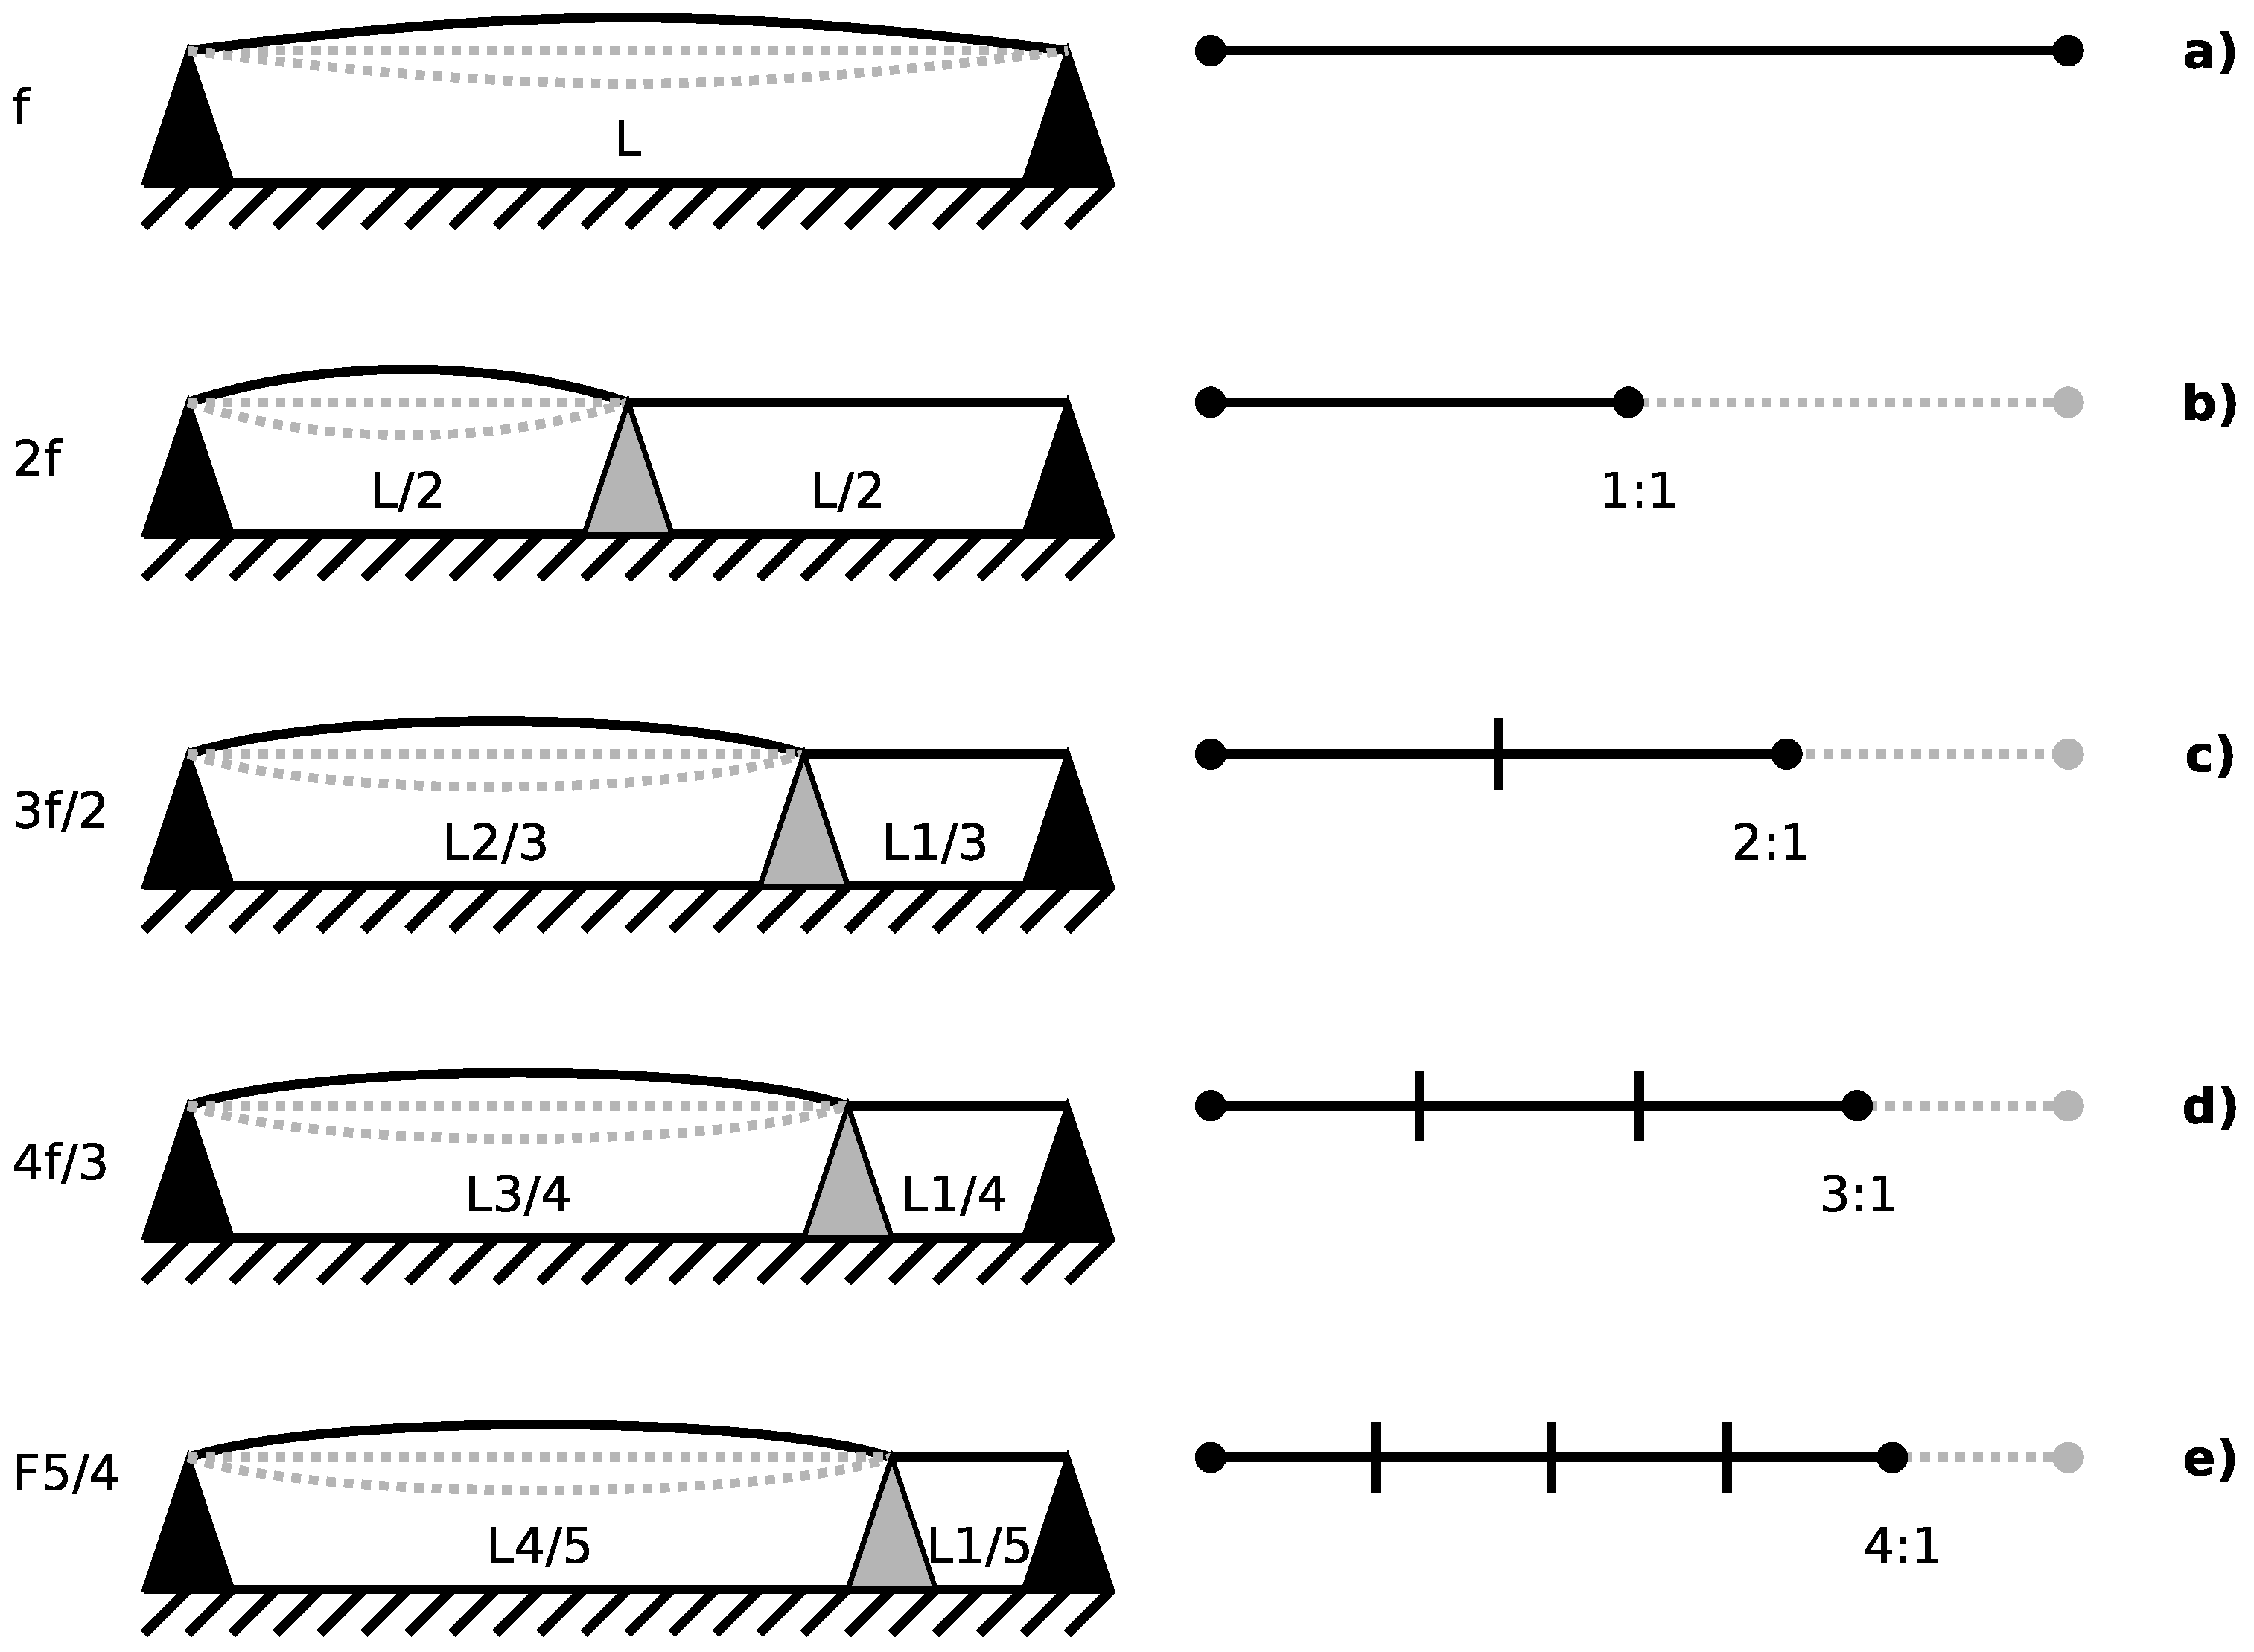
\includegraphics[width=\textwidth]{chapters/cap-musica-composer/consonancia0.eps}
\caption{Consonância entre frequências.}
\label{fig:consonancia}
\end{figure}

Quando a longitude da corda do monocórdio diminui, 
a frequência do som gerado aumenta, é dizer se obtêm tons mais agudos,
tendo longitude e frequência uma relação inversa \cite[pp. 12]{arbones2012armonia}. 
Entre os resultados obtidos com este instrumento, 
está a constatação de que algumas longitudes menores da corda, 
geravam sons mais agradáveis de ouvir, ao ser executados ao mesmo tempo com o som gerado pela corda completa \cite[pp. 12]{arbones2012armonia}.

Assim, os pitagóricos descobriram que as proporções mais simples das cordas,
eram as que geravam os sons mais agradáveis de ouvir \cite[pp. 12]{arbones2012armonia};
nas Figuras \ref{fig:consonancia}[b - e], podemos ver algumas das proporções de longitudes estudadas,
como: 1:1, 2:1, 3:1 e 4:1; que geram tons com frequências: 
$2$f, $\frac{3}{2}$f, $\frac{4}{3}$f e , $\frac{5}{4}$f.
Sendo a relação mais simples (1:1) a que provoca a duplicação da frequência (Figura \ref{fig:consonancia}b),
que na atualidade chamamos \hyperref[sec:pos:Oitava]{\textbf{oitava}}; 
a seguinte em simplicidade é a proporção 2:1 que gera um som com uma frequência de $\frac{3}{2}$f (Figura \ref{fig:consonancia}c),
que na atualidade chamamos de \textbf{intervalo de quinta};
por outro lado, nas Figuras \ref{fig:consonancia}[d-e] com frequências $\frac{4}{3}$f e , $\frac{5}{4}$f respetivamente,
a sensação de consonância diminui proporcionalmente à complexidade das frações das frequências \cite[pp. 12]{arbones2012armonia}.

Por estas observações os pitagóricos concluíram que seriam consonantes com a frequência $f$, sons com uma frequência igual a 
\begin{equation}
\label{eq:simplespita}
\frac{n+1}{n}f,
\end{equation}
sendo que o nível de consonância diminui com o aumento de ``n'' \cite[pp. 14]{arbones2012armonia}.

\PRLsep{Escala diatônica}
\label{ref:paginadiatonicanumerica}

Se usamos as frequências da Equação \ref{eq:simplespita}, para $n=\{1,2,3,4\}$,
e multiplicamos estas frequências por $\frac{3}{2}$ ou $\frac{1}{2}$, que
são as proporções de frequência que geram maior consonância,
obteremos a \hyperref[sec:pos:Diatonica]{\textbf{escala diatônica}} (E.D.).
Esta escala pode ser comparada com a \hyperref[sec:pos:Cromatica]{\textbf{escala cromática}} (E.C.)
que está \hyperref[subsec:tempigual]{\textbf{igualmente temperada}}, 
como mostra a Tabela \ref{tab:pitagorascromatica}, onde foi usada a nota musical ``dó'' como referencia, a \hyperref[sec:Tonica]{\textbf{tônica}}.
\begin{table}[h]
  \centering
  \begin{tabular}{|l|l|l|l|l|l|l|l|l|}
  \hline
  E. Diatônica  & dó & ré & mi & fá & sol & lá & si & dó \\ \hline
  \hline
  Freq. E.D.  & f  & $\frac{9}{8}$f & $\frac{5}{4}$f & $\frac{4}{3}$f & $\mathbf{\frac{3}{2}}$\textbf{f} & $\frac{5}{3}$f & $\frac{15}{8}$f & $\mathbf{2}$\textbf{f}\\ \hline
  E. Cromática & f  & $\alpha^{2}$f  & $\alpha^{4}$f  & $\alpha^{5}$f  & $\alpha^{7}$f  & $\alpha^{9}$f  & $\alpha^{11}$f  & $2$f\\ \hline \hline
  %%Error$\%$ &  0.0  & 0.23 & 0.79  & 0.11 & 0.11 & 0.91 & 0.68 & 0.0 \\ \hline
  Error$\%$ &  0.00 & 3.91 &-13.69 &-1.96 & 1.96 &-15.64&-11.73& 0.00 \\ \hline
  \end{tabular}
  \caption{Relação de frequências, usando $\alpha=2^\frac{1}{12}$.}
  \label{tab:pitagorascromatica}
\end{table}

É possível ver que existe uma ligeira diferença numérica, 
entre as proporções de frequências na escala diatônica baseada nas consonâncias descobertas pela escola pitagórica,
e as proporções de frequência de nossa atual escala cromática igualmente temperada,
no menor dos casos temos um  erro na frequência de $1.96\%$ de um \hyperref[sec:pos:Semitom]{\textbf{semitom}}, 
e no pior dos casos um erro de $15.64\%$.

\PRLsep{Análises objetivo}
Fora da subjetiva perspetiva da escola pitagórica, 
em indicar que frações mais simples na frequência geram sons consonantes; 
existem motivos objetivos para fundamentar esta afirmação.

Na Figura \ref{fig:corda32} podemos ver as sinais $y_{f}$ e $y_{\frac{3}{2}f}$, 
produzidas pelos sons com frequências $f=1000$hz e $\frac{3}{2}f$,
correspondentes a cordas de longitude $L$ e $\frac{2}{3}L$ respetivamente;
é interessante observar que se precisam \textbf{dois} ciclos completos da sinal $y_{f}$,
para que ambas sinais voltem a estar em sincronia e que a sinal soma, $y_{f}+y_{\frac{3}{2}f}$, forme um ciclo completo.


Na mesma linha de análises, na Figura \ref{fig:corda53} podemos observar as sinais $y_{f}$ e $y_{\frac{5}{3}f}$, 
produzidas pelos sons com frequências $f=1000$hz e $\frac{5}{3}f$,
correspondentes a cordas de longitude $L$ e $\frac{3}{5}L$ respetivamente;
e similarmente ao caso anterior, observamos que se precisam \textbf{três} ciclos completos da sinal $y_{f}$,
para que ambas sinais voltem a estar em sincronia e que a sinal soma, $y_{f}+y_{\frac{5}{3}f}$, forme um ciclo completo.

\begin{figure}
    \centering
    \begin{subfigure}[b]{0.8\textwidth}
        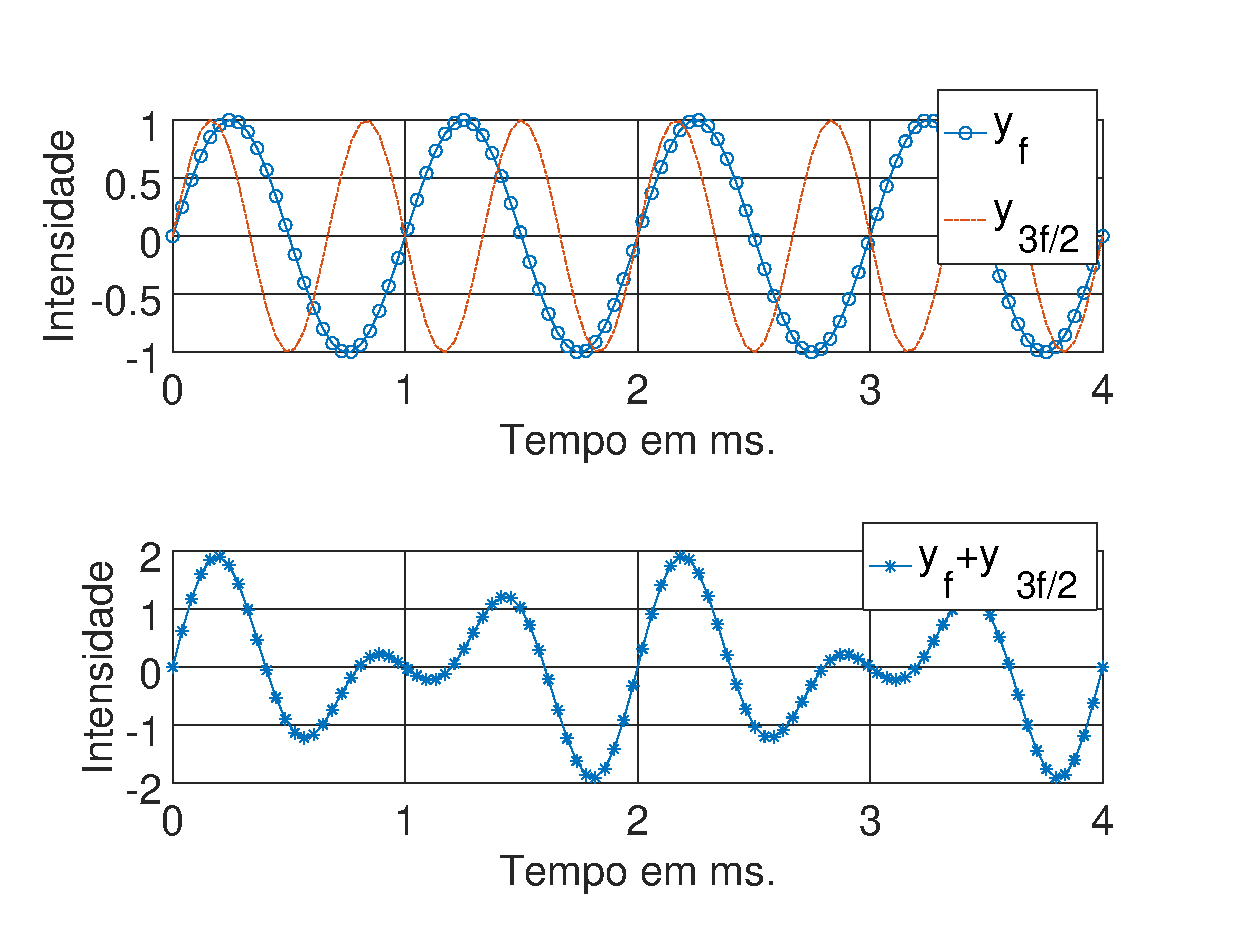
\includegraphics[width=\textwidth]{chapters/cap-musica-composer/consonancia32.eps}
        \caption{Consonância entre sinais com frequências $f$ e $\frac{3}{2}f$}
        \label{fig:corda32}
    \end{subfigure}
    ~ %add desired spacing between images, e. g. ~, \quad, \qquad, \hfill etc. 
      %(or a blank line to force the subfigure onto a new line)
    \begin{subfigure}[b]{0.8\textwidth}
        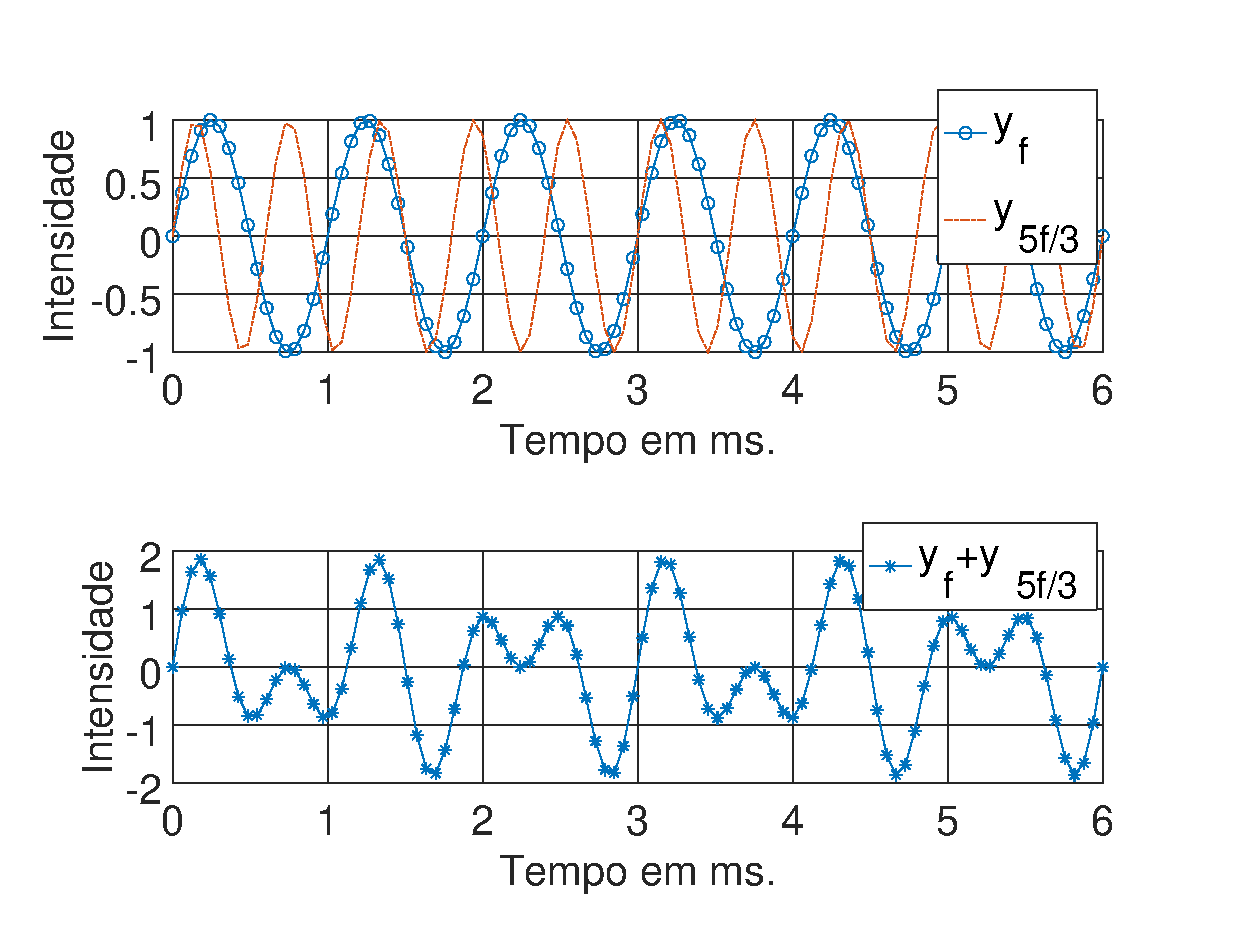
\includegraphics[width=\textwidth]{chapters/cap-musica-composer/consonancia53.eps}
        \caption{Consonância entre sinais com frequências $f$ e $\frac{5}{3}f$}
        \label{fig:corda53}
    \end{subfigure}
\caption{Analises de consonância.}
\label{fig:consonanciaper}
\end{figure}

Assim, deduzimos que pela forma fraccionaria e relativa das frequência nas sinais, 
podemos usar o denominador da fração na frequência,
para conhecer quantos ciclos debem passar para que a ambas sinais em estudo voltem a estar em sincronia;
de modo que seremos capazes de relacionar um estado de maior nível de dissonância (N.D.) com um maior número de ciclos.
A Tabela \ref{tab:pitagorascromatica2} mostra estas relações, 
porém foram agregadas as letras ``a'' e ``b'' para indicar menor e maior dissonância respetivamente,
nos casos com igual N.D., este critério foi aplicado tomando em conta que a escala
que comumente temos num piano está igualmente temperada,
é como vimos na Tabela  \ref{tab:pitagorascromatica},
existe um erro de aproximação a estas frações;
de modo que foi colocada a etiqueta de ``b'' ao caso de maior erro e a etiqueta de ``a'' ao de menor.
\begin{table}[h]
  \centering
  \begin{tabular}{|l|l|l|l|l|l|l|l|l|}
  \hline
  E. Diatônica    & dó & ré & mi & fá & sol & lá & si & dó \\ \hline
  \hline
  Semitons E.C.   & 0  & 2  & 4  & 5  & 7  & 9  & 11 & 12 \\ \hline
  Freq. E.D.  & f  & $\frac{9}{8}$f & $\frac{5}{4}$f & $\frac{4}{3}$f & $\mathbf{\frac{3}{2}}$\textbf{f} & $\frac{5}{3}$f & $\frac{15}{8}$f & $\mathbf{2}$\textbf{f}\\ \hline \hline
  N.D. &  0 & 8a & 4 & 3a & 2 & 3b & 8b & 1 \\ \hline
  \end{tabular}
  \caption{Nível de dissonância com a nota musical dó.}
  \label{tab:pitagorascromatica2}
\end{table}

\begin{example}
Com a ajuda de um piano, que esteja igualmente temperado,
use a nota dó como referencia e comprove o nível de consonância com todas as demais notas musicais;
verifique se concorda com o mostrado na Tabela \ref{tab:pitagorascromatica2}.
\end{example}~

\PRLsep{Conclusões}

Finalmente, podemos concluir que existe uma maior consonância entre
\begin{itemize} 
\item os tons com frequências $f$ e $2f$, e 
\item os tons com frequências $f$ e $\frac{3}{2}f$;
\end{itemize}
para outros valores de frequência, 
como entre $f$ e $\frac{4}{3}f$, o nível de consonância diminui  
 gradualmente com o aumento da complexidade das frações nas frequências.

Na música atual, as relações de consonância são usadas na escala cromática, 
em notas musicais com:
\begin{itemize} 
\item Uma oitava de diferença, para as frequências relacionadas como $f$ e $2f$, 
por exemplo: dó e dó'.
\item Um intervalo de quinta, sete semitons, para frequências relacionadas como  $f$ e $\frac{3}{2}f$, 
por exemplo: dó e sol. Porém, numa escala igualmente temperada, 
os 7 semitons são uma aproximação\footnote{Sim, você está supondo certo,
toda a música atual está ligeiramente ``desafina'', pois usa uma aproximação para a consonância.}
 da fração $\frac{3}{2}$.
\end{itemize}~


Os seres humanos não nos sentimos confortáveis ao terminar o dia com um argumento não resolvido; 
da mesma forma, não apreciamos terminar nossa música com uma dissonância não resolvida \cite[pp. 26]{wright2012essential}.

 

\section{Música tonal, modal e atonal}
\label{sec:ModosEntenderMusica}
Podem existir vários modos de entender a música, como por exemplo o ``tonal'' e o ``modal''.
A diferencia entre estes dois paradigmas da música, 
radica na forma em que a música desenvolve sua existência no tempo \cite[pp. 155]{arbones2012armonia}.


\subsection{Música tonal}
\label{sec:MusicaTonal}
\index{Música!Música tonal}
A música tonal inicia no Barroco, aproximadamente entre os anos 1600 e 1750,
e tem a  caraterística de ser um tipo de  música que se projeta para adiante;
em cada momento da musica tonal, um acorde pelo geral conduz a outro,
pois existe um jogo de tensão e relaxação que deve ser resolvido,
a este rol dos acordes chama-se ``função de acorde'' \cite[pp. 155-156]{arbones2012armonia}.


Na música tonal, 
as notas musicais são organizadas seguindo a importância destas ao redor de uma nota  principal,
que foi batizada como ``tônica'', ou centro tonal \cite[pp. 27]{arbones2012armonia}.
Este ordem segue as regras de \hyperref[ref:paginadiatonicanumerica]{\textbf{consonância}} observadas pela escola pitagórica,
que provoca que as alturas dos tons na \hyperref[sec:pos:Diatonica]{\textbf{escala diatônica}} 
estejam formados usando frações em função de uma frequência fundamental, a tônica.

Mesmo que a disposição fracionaria das notas na música tonal, gere melodias muito consonantes,
problemas\footnote{Problemas na diminuição da consonância; é dizer o aumento da dissonância.} 
podem ser encontrados sim se desenvolvem melodias ao redor de uma nota diferente da tônica;
e dizer, longe da nota musical da qual foram calculadas as demais notas \cite[pp. 28]{arbones2012armonia},
de ali a importância da tônica na música tonal.

\subsubsection{Música tonal desde seculo XX}
A maioria das músicas  escritas desde o seculo XX é diatônica e tonal;
porém, atualmente a música tonal não tem mais a mesma velha definição de tonalidade dos seculos anteriores  \cite[pp. 63]{copland1974ouvir},
em primeiro lugar porque a música atual, geralmente usa instrumentos com \hyperref[subsec:tempigual]{\textbf{temperamento igual}},
o que provoca que não exista uma nota mais importante que as demais, 
pelo que transposições podem ser feitas sem alterar a consonância de uma peça musical.
Outra consequência do \hyperref[subsec:tempigual]{\textbf{temperamento igual}},
é que a o intervalo de quinta considerado antes como de uma consonância perfeita,
com frequências que tem uma proporção 3/2 (1.5), é agora medido com sete semitons (aproximadamente 1.49830707687668),
obtendo desta maneira só uma aproximação à consonância.\\




\subsection{Música modal}
\label{sec:MusicaModal}
\index{Música!Música modal}

No estilo modal o tempo tem se interpretado de dois jeitos diferentes:
\begin{itemize}
\item Como uma eternidade; como por exemplo no canto gregoriano; e dizer 
sem noção de passado, presente ou futuro.
\item Com o tempo como presente continuo, 
o acontecimento sonoro é completo em cada instante; é dizer,
 o sonido atual não esta condicionado ao passado ou ao futuro;
como por exemplo o ``bebop jazz''\cite[pp. 156]{arbones2012armonia}.
\end{itemize}



\subsection{Música atonal: dodecafonismo}
\label{sec:MusicaAtonal}
\index{Música!Música atonal}
O dodecafonismo é uma técnica de composição musical, 
criada na década de 1920 pelo compositor austríaco Arnold Schonberg \cite[pp. 121]{arbones2012armonia}\cite[pp. 263]{holst1998abc}.


A técnica dodecafônica, ou com igualitarismo tonal,
procura a ideia de uma música \textbf{atonal}; é dizer carente de centro tonal,
que se desliga de uma maior gravitação a uma nota, a tônica, sobre as demais;
O dodecafonismo desenvolve um método para evitar a preponderância de uma nota sobre outras,
de modo que todas tem o mesmo valor relativo,
e possam ser apreciadas da mesma forma numa composição musical 
\cite[pp. 122]{arbones2012armonia}.

Para evitar a centralização da peça musical numa nota especifica,
o compositor deve completar ciclos que usem as 12 notas 
(brancas e negras numa oitava nu piano). 
Apos uma nota musical ser usada, 
esta não podia volver a ser usada ate o seguinte ciclo de 12 notas \cite[pp. 123]{arbones2012armonia}.


 
\section{Tônica e dominante}
\index{Música!Tônica}


\subsection{Tônica}
\label{sec:Tonica}
Na \hyperref[sec:MusicaTonal]{\textbf{música tonal}} toda melodia tem uma ``tônica''; 
é dizer, uma nota mais importante \cite[pp. 19]{holst1998abc}, 
pois como é explicado na Seção \ref{sec:consonancia}, se temos uma escala diatônica,
onde as notas são afinadas buscando a \hyperref[ref:consonancia]{\textbf{consonância}},
como foi indicada pela escola pitagórica; então todas as notas são expressadas,
como uma fração de uma nota principal, a tônica. 
Como uma consequência inesperada, deste tipo de afinação, 
qualquer transposição de uma melodia, longe deste centro tonal, 
provocará a introdução de dissonâncias,
a este problema chama-se a ``coma pitagórica'' \cite[pp. 24]{arbones2012armonia}.
 

Do mesmo modo que o sujeito numa oração é identificável, a tônica também é identificável;
no âmbito literário o uso das palavras numa frase, 
provoca que identifiquemos entre elas ao sujeito, pelo papel que esta cumpre na frase.
Acontece da mesma forma na linguagem musical; numa melodia,
a ordem da escolha consecutiva das notas musicais, 
fazem que a tônica seja perceptível, pois dá à melodia ou harmonia, 
seu sentido musical como o centro a onde se converge para dar sentido de finalização a frase \cite[pp. 19]{holst1998abc}.

Assim a tônica é identificável, numa melodia ou harmonia, 
porque esta é geralmente  usada no final  da frase musical, 
quando se quer dar uma sensação de um final forte;
é dizer que expressa claramente a conclusão de uma ideia.
Nesse caso, a tônica comumente é usado apos uma nota que está separada um 
\hyperref[sec:intervalomelodico]{\textbf{intervalo}} de quinta;
chama-se a está nota de \hyperref[sec:dominante]{\textbf{dominante}}.

\subsection{Dominante}
\label{sec:dominante}

O intervalo entre a tônica e a quinta nota musical mais aguda 
(\hyperref[fig:abc-iquinta2]{\textbf{intervalo de quinta}} ascendente), 
na escala diatônica, 
é o intervalo mais importante\footnote{Expeto se a tônica é um si, nesse caso é melhor contar 7 semitons},
pois é o intervalo \hyperref[tab:pitagorascromatica2]{\textbf{mais consonante}}, 
só superado pelo intervalo de oitava. 
Por conta disto o quinto grau dos modos da escala diatônica é chamado  de ``dominante'';
tendo esta uma forte atração com a tônica. 
Esta caraterística é um dos componentes que ajudam a manter interessante  uma melodia \cite[pp. 24]{holst1998abc}.
Na Seção \ref{sec:Cadencia}, onde é tratado o tema da \hyperref[sec:Cadencia]{\textbf{cadência}},
pode ser encontrada mais informação sobre a relação entre a tônica e a dominante.

\subsection{A tônica e as escalas modais}
Qualquer nota da escala diatônica podem ser escolhidas como tônica;
assim, existira para cada uma destas escolhas existirá um distinto grupo de sete notas,
ordenadas em relação a esta tônica. Estos grupos são chamados modos \cite[pp. 21]{holst1998abc};
a Tabela \ref{tab:modosdiatonica}, mostra o nome de todos os modos possíveis da escala diatônica,
e indica com números romanos todos os intervalos possíveis,
de modo que ``I'' indica a tônica, e ``IV'' indica a dominante.

\begin{table}[h]
  \centering
  \begin{tabular}{|l||l|l|l|l|l|l|l|}
  \hline
  Modo      & I   & II  & III & IV  & V   & VI  & VII \\ \hline \hline
  Jônico    & dó  & ré  & mi  & fá  & sol & lá  & si  \\ \hline
  Dórico    & ré  & mi  & fá  & sol & lá  & si  & dó  \\ \hline
  Frígio    & mi  & fá  & sol & lá  & si  & dó  & ré  \\ \hline
  Lídio     & fá  & sol & lá  & si  & dó  & ré  & mi  \\ \hline
  Mixolídio & sol & lá  & si  & dó  & ré  & mi  & fá  \\ \hline
  Eólica    & lá  & si  & dó  & ré  & mi  & fá  & sol \\ \hline
  Lócrio    & si  & dó  & ré  & mi  & fá  & sol & lá  \\ \hline
  \end{tabular}
  \caption{Escalas modais e os graus.}
  \label{tab:modosdiatonica}
\end{table}

\subsection{Nome dos graus na escala diatônica}
A escala diatônica está formada por oito graus, 
sendo que cada um destes tem uma função especifica \cite[pp. 31]{cardoso1973curso};
A Tabela \ref{tab:relacaotonica} mostra todos os nomes para estes graus, 
o grau VIII não foi colocado pois é a repetição do grau I. 
\begin{table}[h]
  \centering
  \begin{tabular}{|l|l|p{7cm}|}
  \hline
  Nome           & Grau & Função\\ \hline \hline
  Tônica         & I    & Repouso natural da tonalidade.\\ \hline
  Supertônica    & II   & Grau acima da tônica.\\ \hline 
  Mediante       & III  & Grau intermediário entre a tônica e a dominante.\\ \hline 
  Subdominante   & IV   & Grau abaixo da dominante.\\ \hline 
  Dominante      & V    & Quinto grau a partir da tônica.\\ \hline 
  Superdominante & VI   & Grau acima da dominante.\\ \hline 
  Sensível       & VII  & Sétimo grau acima da tônica. \\ \hline
  \end{tabular}
  \caption{Nome dos graus nas notas musicais.}
  \label{tab:relacaotonica}
\end{table}


%%%%%%%%%%%%%%%%%%%%%%%%%%%%%%%%%%%%%%%%%%%%%%%%%%%%%%%%%%%%%%%%%%%%%%%%%%%%%%%%
%https://pt.wikipedia.org/wiki/T%C3%B4nica
 
%%%%%%%%%%%%%%%%%%%%%%%%%%%%%%%%%%%%%%%%%%%%%%%%%%%%%%%%%%%%%%%%%%%%%%%%%%%%%%%%
\section{Cadência}
\label{sec:Cadencia}
\index{Música!Cadência}

\begin{tcbinformation}{Música cadenciosa}
\index{Música!Música cadenciosa}
\label{ref:musicacadenciosa}
É aquela que tem um ritmo facilmente apreciável, na qual as terminações, ou seja cadências,
são fáceis de perceber \cite[pp. 60]{pedrell2009diccionario}.
Para que uma música seja cadenciada é preciso que ritmo e harmonia se combinem  
para dar uma sensação de exatidão \cite[pp. 68]{melcior1859diccionario}.
\end{tcbinformation} 


O final da frase musical está marcado pela cadência, 
este nome vem da palavra ``cadenza''  em italiano que significa caindo ou cessando \cite[pp. 34]{bennett1993elementos} \cite[pp. 68]{melcior1859diccionario}. 
As cadências existem nas frases melódicas ou harmônicas, 
e são identificáveis como os períodos de repouso entre as frases musicais;
estas cumprem o mesmo papel que os signos de pontuação na gramática, 
já seja como virgulas, pontos e virgulas, pontos, signos de interrogação
\cite[pp. 66,67]{melcior1859diccionario} \cite[pp. 34]{bennett1993elementos}, 
etc.


%%%%%%%%%%%%%%%%%%%%%%%%%%%%%%%%%%%%%%%%%%%%%%%%%%%%%%%%%%%%%%%%%%%%%%%%%%%%%%%%
\subsection{Cadência harmônica}
\label{sec:CadenciaHarmonica}
\index{Música!Cadência harmônica}

As cadencias harmônicas estão representadas por um par de ``acordes''
que são usados para finalizar uma frase musical, estas tem um sentido de mensagem. 

Entre os tipos de cadencias harmônicas, 
temos as que nos dão a liberdade expressar uma pausa momentânea, suspenso ou o final de uma ideia.

A Tabela \ref{tab:tiposdecadencia} mostra algumas desta opções, 
na primeira coluna temos os nomes dos tipos de cadencias,
na segunda coluna temos a ordem e os graus dos acordes que são usados para gerar essa cadência 
e na terceira coluna está a descrição de cada um dos tipos de cadência.

\begin{table}[h]
  \centering
  \begin{tabular}{|p{4cm}|l|p{8cm}|}
  \hline
  Nome & Acordes   & Analogia \\ \hline
  \hline
  Cadência perfeita & V-I       & Dá sentido de algo perfeitamente acabado, 
  equivalente a um ponto final na gramática \cite[pp. 34]{bennett1993elementos}. \\ \hline
  
  Cadência plagal   & IV-I      & Dá um sentido equivalente a um ponto final na gramática, 
  também é chamado de cadência do ``Amém'' 
  por seu uso em hinos religiosos \cite[pp. 34]{bennett1993elementos} \\ \hline

  Cadência imperfeita ou semicadência \cite[pp. 103]{grabner2001teoria} & ?-V    & Acontece quando se vá de um grau qualquer para finalizar na dominante (V), 
  porém é comum ver que se usam:
  I-V,II-V e IV-V. Esta cadência dá à música a sensação de um final incompleto, 
  seu efeito é similar ao de uma virgula na gramática,
  \cite[pp. 34]{bennett1993elementos}. \\ \hline

  Cadência interrompida & V-($\neq$I) & Acontece quando se sugere que acontecerá uma cadencia V-I (dominante-tônica),
  porém apos V se finaliza em qualquer grau 
  diferente da \hyperref[sec:Tonica]{\textbf{tônica}}, geralmente VI,
  e dá uma sensação de surpresa e de interrupção à música; ou seja uma frase incompleta.
  \cite[pp. 35]{bennett1993elementos}. \\ \hline  
\end{tabular}
  \caption{Tipos de cadência harmônica.}
  \label{tab:tiposdecadencia}
\end{table}

\begin{example}
A Figura \ref{fig:abc-perfeita1} mostra uma cadência perfeita para uma tônica em acorde de dó.
A cadência dá a sensação de uma frase com ponto final.
\end{example}

\begin{figure}[H]
\centering
\begin{abc}[name=abc-perfeita1,width=1.0\linewidth]
X: 1 % start of header
K: C % scale: C major
M: 2/4 %meter - compasso
V:1 %name="Pauta com clave de fá"   sname="Pauta com clave de fá"
[V:1] | [C2 E2 G2] [F2 A2 C'2]| [E2 G2 B2] [G2 B2 D'2]| [F2 A2 C'2] [G2 B2 D'2]| [C2 E2 G2] z2|
w: ~ ~ ~ ~ ~ V I
\end{abc}
\caption{Cadência perfeita.}
\label{fig:abc-perfeita1}
\end{figure}

\begin{example}
A Figura \ref{fig:abc-plagal1} mostra uma cadência plagal para uma tônica em acorde de dó.
A cadência dá a sensação de uma frase com ponto ao  final.
\end{example}

\begin{figure}[H]
\centering
\begin{abc}[name=abc-plagal1,width=1.0\linewidth]
X: 1 % start of header
K: C % scale: C major
M: 2/4 %meter - compasso
V:1 %name="Pauta com clave de fá"   sname="Pauta com clave de fá"
%[V:1] | [E2 G2 B2] [F2 A2 C'2]| [E2 G2 B2] [G2 B2 D'2]| [C2 E2 G2] z2|
[V:1] | [C2 E2 G2] [F2 A2 C'2]| [E2 G2 B2] [G2 B2 D'2]| [E2 G2 B2] [F2 A2 C'2]| [C2 E2 G2] z2|
w: ~ ~ ~ ~ ~ IV I
\end{abc}
\caption{Cadência plagal.}
\label{fig:abc-plagal1}
\end{figure}

\begin{example}
A Figura \ref{fig:abc-imperfeita1} mostra uma cadência imperfeita para uma tônica em acorde de dó.
A cadência dá a sensação de uma frase com um final débil, como de uma mistura de signo de admiração e interrogação.
\end{example}

\begin{figure}[H]
\centering
\begin{abc}[name=abc-imperfeita1,width=1.0\linewidth]
X: 1 % start of header
K: C % scale: C major
M: 2/4 %meter - compasso
V:1 %name="Pauta com clave de fá"   sname="Pauta com clave de fá"
[V:1] | [C2 E2 G2] [F2 A2 C'2]| [E2 G2 B2] [G2 B2 D'2]| [E2 G2 B2] [F2 A2 C'2]| [G2 B2 D'2] z2|
w: ~ ~ ~ ~ ~ IV V
\end{abc}
\caption{Cadência imperfeita.}
\label{fig:abc-imperfeita1}
\end{figure}


\begin{example}
A Figura \ref{fig:abc-interrompida1} mostra uma cadência interrompida para uma tônica em acorde de dó.
A cadência dá a sensação de uma frase incompleta.
\end{example}

\begin{figure}[H]
\centering
\begin{abc}[name=abc-interrompida1,width=1.0\linewidth]
X: 1 % start of header
K: C % scale: C major
M: 2/4 %meter - compasso
V:1 %name="Pauta com clave de fá"   sname="Pauta com clave de fá"
[V:1] | [C2 E2 G2] [F2 A2 C'2]| [E2 G2 B2] [G2 B2 D'2]| [E2 G2 B2] [G2 B2 D'2]| [A2 C'2 E'2] z2|
w: ~ ~ ~ ~ ~ V VI
\end{abc}
\caption{Cadência interrompida.}
\label{fig:abc-interrompida1}
\end{figure}

%%%%%%%%%%%%%%%%%%%%%%%%%%%%%%%%%%%%%%%%%%%%%%%%%%%%%%%%%%%%%%%%%%%%%%%%%%%%%%%%
\subsection{Cadência melódica} 
\label{subsec:cadenciamelodica}
Quando nos referimos à forma em que uma melodia é finalizada,
estamos falando da cadencia melódica; esta pode ser categorizada em: 
\begin{itemize}
\item \textbf{Cadências}, se o repouso é equivalente a um ponto na gramática \cite[pp. 66,67]{melcior1859diccionario},
como o produzido por uma dominante (V) seguida de um tônica (I).
\item \textbf{Semicadências}, se repouso é equivalente a um ponto e virgula na gramática \cite[pp. 66,67]{melcior1859diccionario};
esta também é chamada de cadencia imperfeita e se carateriza por terminar numa dominante (V) 
que geralmente vem precedida por  I, II ou IV \cite[pp. 103]{grabner2001teoria}; 
é possível ver este tipo de cadencia no final da frase antecedente de um 
\hyperref[sec:Periodo]{\textbf{período}} \cite[pp. 21]{latham2008diccionario}.
\item \textbf{Quartos de cadência}, se o repouso é igual a uma virgula \cite[pp. 66,67]{melcior1859diccionario}.
\end{itemize}~

Todas estas cadencias dão à melodia uma sensação da conclusão de uma ideia; 
porém, cada uma destas nos deixa uma perspetiva diferente sobre o que vem depois e quando.

Além dos tipos de cadencias melódicas anteriormente mencionadas, podemos achar também a:
\begin{itemize}
\item \textbf{Cadência interrompida}, este tipo de cadencia se verifica 
quando ao final de um período sugerimos que iremos de 
\hyperref[sec:dominante]{\textbf{dominante}} a \hyperref[sec:Tonica]{\textbf{tônica}},
porém terminamos em qualquer outro grau; ou seja pulamos da dominante a um grau diferente da tônica 
\cite[pp. 67]{melcior1859diccionario} \cite[pp. 60]{pedrell2009diccionario}. 
\end{itemize}~

Em geral veremos um uso aprimorado das cadências, na frase consequente de um \hyperref[sec:Periodo]{\textbf{período}},
onde o tipo do cadência ajudará a expressar o uso que esta terá na peça musical  \cite[pp. 66,67]{melcior1859diccionario}.

\begin{example}
A Figura \ref{fig:abc-frasemelodica1} mostra duas frases com tônica em dó, 
a primeira frase com uma semicadencia (VI-V) e a segunda frase com uma cadência (V-I).
\end{example}

\begin{figure}[H]
\centering
    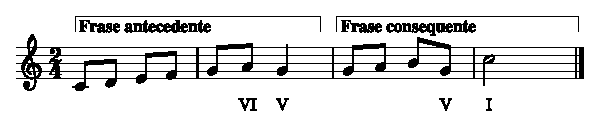
\includegraphics[width=\textwidth]{chapters/cap-musica-composer/frasemelodica1-1.eps}
\caption{Duas frases melódicas com tônica em dó.}
\label{fig:abc-frasemelodica1}
\end{figure}

\begin{example}
A Figura \ref{fig:abc-frasemelodica2} mostra duas frases  com tônica em sol, 
a primeira frase com uma cadência interrompida (V-III) e a segunda frase com uma cadência (V-I).
\end{example}

\begin{figure}[H]
\centering
    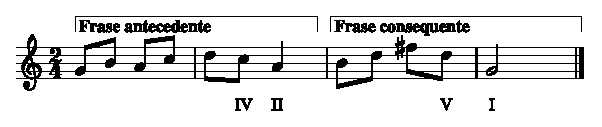
\includegraphics[width=\textwidth]{chapters/cap-musica-composer/frasemelodica2-1.eps}
\caption{Duas frases melódicas com tônica em sol.}
\label{fig:abc-frasemelodica2}
\end{figure}
% https://es.wikipedia.org/wiki/Cadencia_(música)

% https://en.wikipedia.org/wiki/Cadence



%%%%%%%%%%%%%%%%%%%%%%%%%%%%%%%%%%%%%%%%%%%%%%%%%%%%%%%%%%%%%%%%%%%%%%%%%%%%%%%%
\section{Articulação}
\label{sub:Articulação}
\index{Música!Articulação}

Nas partituras podemos ver alguns símbolos, 
que o compositor coloca como indicação ao interprete,
para informar como as notas musicais devem ser executadas ou 
articuladas entre sim \cite[pp. 56]{alves2004teoria}.
%%%%%%%%%%%%%%%%%%%%%%%%%%%%%%%%%%%%%%%%%%%%%%%%%%%%%%%%%%%%%%%%%%%%%%%%%%%%%%%%
\subsection{Legato ou ligadura de expressão}
\label{subsec:Legato}
\index{Música!Legato}
O  ``legato'' é um símbolo  que indica uma ligadura de expressão entre as notas,
neste caso a informação que da o compositor é que as
notas devem ser executadas sem interrupções,
criando uma mudança de tons gradual para passar de uma nota musical a outra \cite[pp. 56]{alves2004teoria}.

\begin{example}
A Figura \ref{fig:legato1} mostra um exemplo de uso do legato. 
Alguns instrumentos podem facilmente articular um legato, por exemplo o violino.
\end{example}

\begin{figure}[h!]
\centering
\begin{abc}[name=abc-legato1,width=0.80\linewidth]
X: 1 % start of header
K: C % scale: C major
M: 2/4 %meter - compasso
 (G2 E2 | G1  A1  G1 E1 )|
\end{abc}
\caption{Melodia com notas que devem ser executadas de forma ligada.}
\label{fig:legato1}
\end{figure}

%%%%%%%%%%%%%%%%%%%%%%%%%%%%%%%%%%%%%%%%%%%%%%%%%%%%%%%%%%%%%%%%%%%%%%%%%%%%%%%%
\subsection{Staccato}
\label{subsec:Staccato}
\index{Música!Staccato}

O staccato é um símbolo, desenhado com um ponto (.), 
que indica a diminuição na \hyperref[sec:pos:Duracion]{\textbf{duração}} de uma nota (aproximadamente um 50\%), 
dando nela um efeito de separação ou destaque \cite[pp. 56]{alves2004teoria}.

\begin{example}
A Figura \ref{fig:staccato1a} mostra um exemplo de uso do staccato. 
Na Figura \ref{fig:staccato1b} podemos ver uma escrita equivalente, sem o uso do símbolo de staccato.
\end{example}

\begin{figure}[h!]
\centering
\begin{subfigure}[c]{0.80\textwidth}
\begin{abc}[name=abc-staccato1a]
X: 1 % start of header
K: C % scale: C major
M: 2/4 %meter - compasso
 .G2 .E2 | .G1  .A1  .G1 .E1 | 
\end{abc}
\caption{Notação de notas musicais em staccato.}
\label{fig:staccato1a}
\end{subfigure}
~ %
\begin{subfigure}[c]{1.00\textwidth}
\begin{abc}[name=abc-staccato1b]
X: 1 % start of header
K: C % scale: C major
M: 2/4 %meter - compasso
 G1 z1 E1 z1 | G1/2 z1/2 A1/2 z1/2 G1/2 z1/2 E1/2 z1/2 | 
\end{abc}
\caption{Forma de execução de notas musicais em staccato.}
\label{fig:staccato1b}
\end{subfigure}
\caption{Melodia com notas que devem ser executadas em staccato.}
\label{fig:staccato1}
\end{figure}

\subsubsection{Staccatissimo}

O staccatissimo, staccato seco ou martelado é um símbolo, com uma função similar ao staccato;
porem indica uma diminuição maior na \hyperref[sec:pos:Duracion]{\textbf{duração}} de nota (aproximadamente ao 25\%) \cite[pp. 56]{alves2004teoria}.

\begin{example}
A Figura \ref{fig:staccatissimo1a} mostra um exemplo de uso do staccatissimo. 
Na Figura \ref{fig:staccatissimo1b} podemos ver uma escrita equivalente, sem o uso do símbolo de staccatissimo.
\end{example}

\begin{figure}[h!]
\centering
\begin{subfigure}[c]{0.80\textwidth}
\begin{abc}[name=abc-staccatissimo1a]
X: 1 % start of header
K: C % scale: C major
M: 2/4 %meter - compasso
 !wedge!G2 !wedge!E2 | !wedge!G1  !wedge!A1  !wedge!G1 !wedge!E1 | 
\end{abc}
\caption{Notação de notas musicais em staccatissimo.}
\label{fig:staccatissimo1a}
\end{subfigure}
~ %
\begin{subfigure}[c]{1.00\textwidth}
\begin{abc}[name=abc-staccatissimo1b]
X: 1 % start of header
K: C % scale: C major
M: 2/4 %meter - compasso
 G1/2 z3/2 E1/2 z3/2 | G1/4 z3/4 A1/4 z3/4 G1/4 z3/4 E1/4 z3/4 | 
\end{abc}
\caption{Forma de execução de notas musicais em staccatissimo.}
\label{fig:staccatissimo1b}
\end{subfigure}
\caption{Melodia com notas que devem ser executadas em staccato.}
\label{fig:staccatissimo1}
\end{figure}

%%%%%%%%%%%%%%%%%%%%%%%%%%%%%%%%%%%%%%%%%%%%%%%%%%%%%%%%%%%%%%%%%%%%%%%%%%%%%%%%
\subsection{Tenuto ou sostenuto}
\label{subsec:Tenuto}
\index{Música!Tenuto}

O tenuto é um símbolo, desenhado com uma linha reta (-), 
que indica que deve ser sustentada a 
\hyperref[sec:pos:Duracion]{\textbf{duração}} e a \hyperref[sec:pos:Intensidade]{\textbf{intensidade}} da nota ao máximo \cite[pp. 56]{alves2004teoria}.

\begin{example}
A Figura \ref{fig:tenuto1} mostra um exemplo de uso do tenuto. 
\end{example}


\begin{figure}[h!]
\centering
\begin{abc}[name=abc-tenuto1,width=0.80\linewidth]
X: 1 % start of header
K: C % scale: C major
M: 2/4 %meter - compasso
 !tenuto!G2 !tenuto!E2 | !tenuto!G1  !tenuto!A1  !tenuto!G1 !tenuto!E1 |
\end{abc}
\caption{Melodia com notas que devem ser executadas de forma sustenido.}
\label{fig:tenuto1}
\end{figure}

%%%%%%%%%%%%%%%%%%%%%%%%%%%%%%%%%%%%%%%%%%%%%%%%%%%%%%%%%%%%%%%%%%%%%%%%%%%%%%%%
\subsection{Accénto}
\label{subsec:Accento}
\index{Música!Accénto}

O accénto é um símbolo, desenhado com  (>), 
que indica que a nota deve ser acentuada; 
é dizer, esta deve receber um aumento de \hyperref[sec:pos:Intensidade]{\textbf{intensidade}} \cite[pp. 56]{alves2004teoria}.

\begin{example}
A Figura \ref{fig:accento1} mostra um exemplo de uso do accénto.
Onde os tempos fracos tem um aumento de intensidade provocando \hyperref[sec:contratempo]{\textbf{contratempos}}. 
\end{example}


\begin{figure}[h!]
\centering
\begin{abc}[name=abc-accento1,width=0.80\linewidth]
X: 1 % start of header
K: C % scale: C major
M: 2/4 %meter - compasso
 G2 !>!E2 | G1  !>!A1  !>!G1 !>!E1 |
\end{abc}
\caption{Melodia com notas que devem ser executadas de forma sostenida.}
\label{fig:accento1}
\end{figure}
 
\section{Recursos rítmico-melódicos}
\begin{tcbinformation}{Ideia musical}
\index{Música!Ideia musical}
\label{ref:ideiamusical}
É uma melodia pequena e muito simples  que não contem recheio né redundâncias obvias \cite[pp. 12]{howard1991aprendendo},
uma ideia pode virar facilmente num \hyperref[sec:Motivo]{\textbf{motivo}} ou uma \hyperref[sec:Frase]{\textbf{frase}} 
se esta cumpre com as suas respetivas definições.
\end{tcbinformation} 

Existem vários recursos rítmicos e melódicos aplicáveis sobre uma ideia musical
que lhe proporcionam maior interesse e a apresentam de novas formas.
Nas seguintes subseções serão apresentados alguns dos recursos mais comuns,
com este fim é usada como origem a ideia musical mostrada na Figura \ref{ritmo:ideiamusical1}. 
\begin{figure}[H]
\centering
\begin{abc}[name=abc-ideiamusical1,width=0.8\linewidth,options={-O= -c -s 1.5}]
X: 1 % start of header
K: C % scale: C major
M: 2/4 %meter - compasso
V:1 %name="Pauta com clave de fá"   sname="Pauta com clave de fá"
[V:1] G1 E1 G1/2 G3/2| A1 G2 F1|
\end{abc}
\caption{Idéia musical.}
\label{ritmo:ideiamusical1}
\end{figure}

%%%%%%%%%%%%%%%%%%%%%%%%%%%%%%%%%%%%%%%%%%%%%%%%%%%%%%%%%%%%%%%%%%%%%%%%%%%%%%%%
\subsection{Sequencia}
\index{Música!Sequencia}
Uma ideia musical pode ser imediatamente repetida 
com uma transposição a uma altura maior ou menor 
\cite[pp. 30]{bennett1993elementos} \cite[pp. 763]{apel1969harvard}.

A Figura \ref{ritmo:sequence-ex1} mostra o uso da ideia musical 
presentada na Figura \ref{ritmo:ideiamusical1} numa sequencia ascendente correspondente a um tom.
\begin{figure}[H]
\centering
    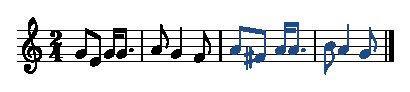
\includegraphics[width=\textwidth]{chapters/cap-musica-composer/sequence-ex1-1.eps}
\caption{Sequencia a partir de uma ideia musical.}
\label{ritmo:sequence-ex1}
\end{figure}

%%%%%%%%%%%%%%%%%%%%%%%%%%%%%%%%%%%%%%%%%%%%%%%%%%%%%%%%%%%%%%%%%%%%%%%%%%%%%%%%
\subsection{Inversão : Reflexão sobre um eixo vertical}
\label{subsec:inversaovertical}
\index{Música!Inversão}

Uma ideia musical pode ser invertida, é dizer escrita ao contrario ao redor de um ponto de pivote;
de modo que as notas com alturas descendentes passam a ser ascendentes, e vice-versa
\cite[pp. 30]{bennett1993elementos}.

A Figura \ref{ritmo:invert-ex1} mostra a inversão, ao redor da nota ``dó'', 
da ideia musical apresentada na Figura \ref{ritmo:ideiamusical1}.
\begin{figure}[H]
\centering
    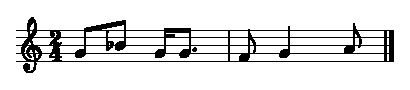
\includegraphics[width=0.8\textwidth]{chapters/cap-musica-composer/invert-ex1-1.eps}
\caption{Inversão de uma ideia musical.}
\label{ritmo:invert-ex1}
\end{figure}


%%%%%%%%%%%%%%%%%%%%%%%%%%%%%%%%%%%%%%%%%%%%%%%%%%%%%%%%%%%%%%%%%%%%%%%%%%%%%%%%
\subsection{Retrogradação : Reflexão sobre um eixo horizontal}
\index{Música!Retrogradação}

Uma ideia musical pode ser escrita em sentido inverso, 
é dizer esta é rescrita iniciando desde a última nota até a primeira em sequencia contraria 
\cite[pp. 77]{arbones2012armonia}.

A Figura \ref{ritmo:retrogrado-ex1} mostra a retrogradação
da ideia musical apresentada na Figura \ref{ritmo:ideiamusical1}.
\begin{figure}[H]
\vspace{-5px}
\centering
    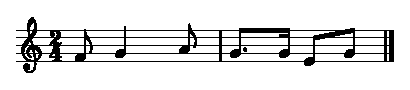
\includegraphics[width=0.8\textwidth]{chapters/cap-musica-composer/retrogrado-ex1-1.eps}
\vspace{-5px}
\caption{Retrogradação de uma ideia musical.}
\label{ritmo:retrogrado-ex1}
\end{figure}


%%%%%%%%%%%%%%%%%%%%%%%%%%%%%%%%%%%%%%%%%%%%%%%%%%%%%%%%%%%%%%%%%%%%%%%%%%%%%%%%
\subsection{Diminuição}
\index{Música!Diminuição}

Uma ideia musical pode ser diminuida, é dizer escrita com durações menores
\cite[pp. 30]{bennett1993elementos}.

A Figura \ref{ritmo:diminuicao-ex1} mostra a diminuição, pela divisão entre dois das durações, 
da ideia musical apresentada na Figura \ref{ritmo:ideiamusical1}.
\begin{figure}[H]
\vspace{-5px}
\centering
    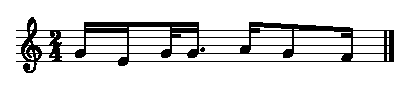
\includegraphics[width=0.8\textwidth]{chapters/cap-musica-composer/diminuicao-ex1-1.eps}
\vspace{-5px}
\caption{Diminuião de uma ideia musical.}
\label{ritmo:diminuicao-ex1}
\end{figure}

%%%%%%%%%%%%%%%%%%%%%%%%%%%%%%%%%%%%%%%%%%%%%%%%%%%%%%%%%%%%%%%%%%%%%%%%%%%%%%%%
\subsection{Aumentação}
\index{Música!Aumentação}

Uma ideia musical pode ser aumentada, é dizer escrita com durações maiores
\cite[pp. 30]{bennett1993elementos}.

A Figura \ref{ritmo:aumentacao-ex1} mostra a aumentação, pelo incremento por dois das durações, 
da ideia musical apresentada na Figura \ref{ritmo:ideiamusical1}.
\begin{figure}[H]
\centering
    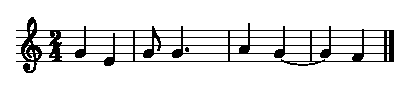
\includegraphics[width=0.8\textwidth]{chapters/cap-musica-composer/aumentacao-ex1-1.eps}
\caption{Aumentação de uma ideia musical.}
\label{ritmo:aumentacao-ex1}
\end{figure}

%%%%%%%%%%%%%%%%%%%%%%%%%%%%%%%%%%%%%%%%%%%%%%%%%%%%%%%%%%%%%%%%%%%%%%%%%%%%%%%%
\subsection{Decoração}
\index{Música!Decoração}

Uma ideia musical pode ser decorada, é dizer podem ser acrescentadas notas ou ornamentos
\cite[pp. 30]{bennett1993elementos}.

A Figura \ref{ritmo:decoracao-ex1} mostra a decoração, pelo aumento de apojaturas e uma linha de expressão, 
na ideia musical apresentada na Figura \ref{ritmo:ideiamusical1}.
\begin{figure}[H]
\centering
    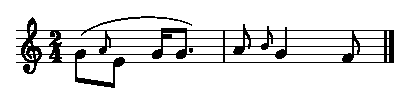
\includegraphics[width=0.8\textwidth]{chapters/cap-musica-composer/decoracao-ex1-1.eps}
\caption{Decoração de uma ideia musical.}
\label{ritmo:decoracao-ex1}
\end{figure}




%%%%%%%%%%%%%%%%%%%%%%%%%%%%%%%%%%%%%%%%%%%%%%%%%%%%%%%%%%%%%%%%%%%%%%%%%%%%%%%%
\section{Motivos}
\label{sec:Motivo}
\index{Música!Motivos}
\index{Música!Motif}
\index{Música!Motiv}

Na literatura sobre música podemos achar  termos, motiv (em alemão) ou motif (em inglês),
para designar ao que no português chamaríamos como motivo \cite[pp. 984]{latham2008diccionario}.
Um motivo é uma unidade melódica curta que se repete ao longo de uma composição musical \cite[pp. 545]{apel1969harvard},
esta tem como intenção proporcionar integração, relação, coerência, lógica, 
compreensão e fluidez ao discurso musical \cite[pp. 984]{latham2008diccionario};
sendo estes usados como elementos básicos para a construção
de temas e linhas melódicas \cite[pp. 984]{latham2008diccionario}.

Os motivos são geralmente mais pequenos que um tema ou uma frase,
podendo ter tamanhos tão pequenos quanto só duas notas,
se estas forem o suficientemente representativas \cite[pp. 545]{apel1969harvard}.

%Los *Leitmotiven (motivos principales) de Wagner son el ejemplo más común
%de ideas musicales concisas que además de proporcionar un elemento 
%de estabilidad en la continuidad musical, contribuyen directamente al desarrollo coherente
%de la acción dramática  \cite[pp. 545]{apel1969harvard}.

\begin{example}
Um exemplo muito interessante de uso de motivos pode ser visto na sinfonia n. 5, op. 67, 
de Ludwig van Beethoven.
Na Figura \ref{fig:10Symphony5Op67}, podemos ver os 10 primeiros compassos da sinfonia,
numa versão simplificada que usa só 3 instrumentos, 2 violinos e uma viola.
Nesse fragmento é identificável o motivo nos dois primeiros compassos,
com um conjunto de notas correspondentes a ``sol~sol~sol~mi$\flat$''.
Nos seguintes 3 compassos, o mesmo motivo é usado, 
mas este sofre uma diminuição de 1 tom na altura de todas as notas, 
além de que a última nota musical sofre um amento na sua duração. 
Finalmente nos últimos 5 compassos, cada instrumento por separado sofre uma diferente mutação do motivo;
o violino 1, usa o motivo com um ganho de 8 semitons e um pequeno aumento da ultima nota;
a viola, usa o motivo com um ganho de 13 semitons e um aumento considerável da última nota; e
o violino 2, usa o motivo com um importante aumento na longitude da última nota.
\end{example}


\begin{figure}[!h]
  \centering
    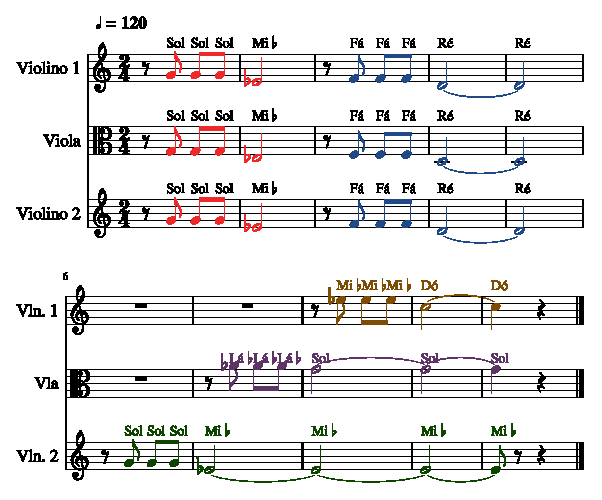
\includegraphics[width=\workboxsize]{chapters/cap-musica-composer/Symphony5Op67-out-1.eps}
\caption{Dez compassos da sinfonia no. 5, op. 67, de Ludwig van Beethoven.}
\label{fig:10Symphony5Op67}
\end{figure}

~


\begin{example}
Na música ``Tico-tico no fubá'' de Zequinha de Abreu, podemos achar exemplos do uso de motivos. 
Na Figura \ref{fig:Tico-tico_no_fuba-1}, temos 5 compassos desta música,
numa versão que usa só 1 instrumentos (um bandolim).
Nesse fragmento é identificável o motivo nos dois primeiros compassos, 
nas 6 primeiras notas musicais, ``mi~ré~mi~fá~mi~lá$\#$''.
imediatamente depois o motivo se repete, porém mudando a ultima nota ate um ``sol$\#$'';
finalmente o motivo volta a parecer, só que além da modificação na altura na ultima nota a um ``ré'',
a duração é encurtada e mais 6 notas musicais são agregadas.
Esta recorrência no uso deste motivo e outros podem ser vistos ao longo de toda a peça musical;
assim, animamo ao leitor a procurar e ouvir a música completa, e tentar identificar o motivo e suas mutações. 
\end{example}

\begin{figure}[!h]
  \centering
    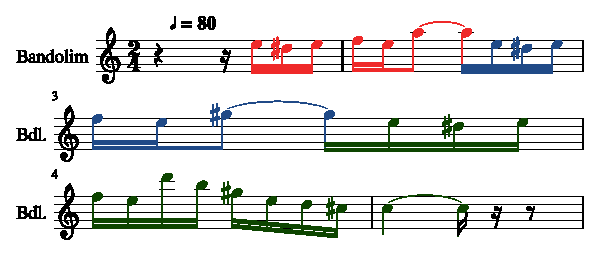
\includegraphics[width=\workboxsize]{chapters/cap-musica-composer/Tico-tico_no_fuba-1.eps}
\caption{Cinco compassos da música ``Tico-tico no fubá'' de Zequinha de Abreu.}
\label{fig:Tico-tico_no_fuba-1}
\end{figure}

~

 
%%%%%%%%%%%%%%%%%%%%%%%%%%%%%%%%%%%%%%%%%%%%%%%%%%%%%%%%%%%%%%%%%%%%%%%%%%%%%%%%
\section{Frase}
\label{sec:Frase}
\index{Música!Frase}
Uma frase é uma unidade musical com sentido e conclusão;
é formada por um grupo de notas que nos dão impressão de que todas pertencem a um mesmo conjunto,
e se caraterizada pela relação entre melodia, ritmo e harmonia,
que termina numa \hyperref[sec:Cadencia]{\textbf{cadência}} \cite[pp. 624]{latham2008diccionario} \cite[pp. 335]{medteoria} \cite[pp. 34]{bennett1993elementos};
é dizer o final da frase pode ser percebido porque a ideia completou o sentido, 
e finaliza num repouso ou uma cadência, além de que a frase seguinte presenta um contraste por estar expressando outra ideia.

\PRLsep{Longitude e usos}

As frases musicais se combinam para formar outras unidades mais longas e completas, 
denominadas \hyperref[sec:Periodo]{\textbf{periodos}} \cite[pp. 624]{latham2008diccionario}.
De forma geral as melodias são construídas usando frases musicais sujeitas a determinadas
regras, de forma similar a como articulamos frases na linguagem falada \cite[pp. 334]{medteoria}.


A longitude de uma frase pode variar, 
porém é comum ver que as frases tem
\begin{itemize}
\item 4 \hyperref[sec:compaso]{\textbf{compassos}} \cite[pp. 624]{latham2008diccionario} \cite[pp. 34]{bennett1993elementos}, 
ou também 
\item 8 compassos  \cite[pp. 335]{medteoria} \cite[pp. 34]{bennett1993elementos};
\end{itemize}
também é comum perceber que as frases que terminam deixando uma sensação de ambiguidade, 
tendem a continuar com outra frase de resposta da mesma longitude \cite[pp. 624]{latham2008diccionario}.


\begin{tcbinformation}
\label{ref:PontoCulminanteSuperior} 
\index{Música!Ponto culminante superior}
\index{Música!PCS}
\index{Música!Clímax}
\textbf{Ponto culminante superior vs. clímax:}
Toda melodia tem uma nota com maior tom (mais aguda), que geralmente está próxima ao final da frase musical;
esta nota é denominada como ponto culminante superior \cite[pp. 336]{medteoria}.
Por outro lado alguns autores fazem uma diferencia entre,
o ponto \textbf{culminante superior} (PCS) e o clímax (Ponto culminante máximo);
onde em cada fragmento da melodia pode ser identificado um PCS,
porém o \textbf{clímax} é a nota mais alta da melodia, como um todo, 
com a característica que a nota é única e está próxima ao final \cite[pp. 12]{melos2012} \cite{HARTMANN2013} \cite[pp. 50]{holland2013music}.
\label{ref:climax}
\end{tcbinformation} 

\PRLsep{Notação}

Na notação musical, 
o compositor pode indicar uma frase, agrupando todas as figuras musicais pertencentes a esta, 
com um símbolo de ligadura escrito acima ou abaixo das notas musicais, 
este simbolo é chamado de ligadura fraseológica \cite[pp. 49]{medteoria} 
\cite[pp. 624]{latham2008diccionario} \cite[pp. 34]{bennett1993elementos}.

A Figura \ref{ritmo:ex2frasesmusicais1} mostra um exemplo de duas frases musicais indicadas pelo uso do simbolo de ligadura.
\begin{figure}[H]
\centering
\begin{abc}[name=abc-ex2frasesmusicais1,options={-O= -c -s 1.5}]
X: 1 % start of header
K: C % scale: C major
M: 4/4 %meter - compasso
V:1 %name="Pauta com clave de fá"   sname="Pauta com clave de fá"
[V:1] (B2 A2 G2 F2| G3 A1 B2 F2) |(C'2 B2 A2 G2| F8)|
\end{abc}
\caption{Duas frases msuicais de 2 compassos cada um.}
\label{ritmo:ex2frasesmusicais1}
\end{figure}

\PRLsep{Estrutura interna}

As frases musicais também podem ser formadas por 2 ou 3 semifrases \cite[pp. 335]{medteoria}.
Com diferencia das frases, que tendem a ser contrastantes; 
as semifrases são identificáveis pois tendem a ser semelhantes entre sim.

\PRLsep{Tipos de frases}

\begin{description}
\item[Frase melódica:]  é uma frase musical formada por um conjunto de tons,
este tipo de frase forma parte de uma linha melódica. 
\item[Frase rítmica:] é uma frase musical formada unicamente por uma distribuição de tempos (ritmo),
este tipo de frase pode ser extraída de um frase melódica, ou servir de base;
também encontraremos frases rítmicas na descrição do ritmo de instrumento de percussão.
\end{description}~

\PRLsep{Frases e texturas musicais}

Na música com \hyperref[subsec:polifonica]{\textbf{textura polifônica}}, 
as frases das diversas linhas melódicas, 
geralmente não finalizam (\hyperref[sec:Cadencia]{\textbf{cadenciam}}) simultaneamente;
por outro lado nas músicas com \hyperref[subsec:homofonica]{\textbf{textura homofônica}},
onde existe uma única linha melódica,
a harmonia de acompanhamento cadência simultaneamente com a melodia \cite{AFraseMelodicaDeterminantes}.

\begin{tcbattention}
Na música contrapontística, é dizer com \hyperref[subsec:polifonica]{\textbf{textura polifônica}}, 
as frases musicais das diferentes vozes se sobrepõem,
com exceção das cadências más importantes onde convergem \cite[pp. 624]{latham2008diccionario}.
\end{tcbattention}

%Na música polifônica há uma distinção maior entre Frase Melódica e Frase estrutural


%%%%%%%%%%%%%%%%%%%%%%%%%%%%%%%%%%%%%%%%%%%%%%%%%%%%%%%%%%%%%%%%%%%%%%%%%%%%%%%%
\subsection{Inicio da frase musical}
\label{subsec:InicioFraseMusical}
O inicio de um ritmo pode ter três formas \cite[pp. 147]{medteoria}:
\begin{itemize}
\item Tético
\item Anacrústico ou protético
\item Acéfalo ou decapitado
\end{itemize}

\subsubsection{Ritmo tético}
\label{subsub:Tetico}
\index{Música!Tético}
É chamado do ritmo tético se este inicia no primeiro tempo do compasso, 
é dizer no tempo forte \cite[pp. 147]{medteoria}.
A Figura \ref{ritmo:iniciotetico1} mostra um exemplo de ritmo tético.
\begin{figure}[H]
\centering
\begin{abc}[name=abc-iniciotetico1]
X: 1 % start of header
K: C % scale: C major
M: 2/4 %meter - compasso
V:1 %name="Pauta com clave de fá"   sname="Pauta com clave de fá"
[V:1] "Compasso 1"G1/2 A B1/2 B1 A1| "Compasso 2"B1 B/2 A/2 G2 |
\end{abc}
\caption{Ritmo tético.}
\label{ritmo:iniciotetico1}
\end{figure}

\subsubsection{Ritmo anacrústico ou protético}
\label{subsub:anacrustica}
\index{Música!Anacrústico}
\index{Música!Protético}
É chamado do ritmo anacrústico ou protético se este inicia antes 
do  tempo forte do compasso \cite[pp. 147-148]{medteoria}.
Na contagem de compassos do ritmo, se diz que este inicia no compasso 1 (primeiro compasso) \cite[pp. 147]{medteoria}.
A Figura \ref{ritmo:anacrustico1} mostra um exemplo de ritmo anacrústico.
\begin{figure}[H]
\centering
\begin{abc}[name=abc-anacrustico1,width=0.8\linewidth]
X: 1 % start of header
K: C % scale: C major
M: 2/4 %meter - compasso
V:1 %name="Pauta com clave de fá"   sname="Pauta com clave de fá"
[V:1]   G1/2 A1/2| "Compasso 1"B1 B/2 A/2 G2 |
\end{abc}
\caption{Ritmo anacrústico.}
\label{ritmo:anacrustico1}
\end{figure}
Não são grafadas as pausas antes da anacruse.
É chamado \textbf{anacruse} às figuras musicais que que estão 
antes do primeiro tempo forte do ritmo, \cite[pp. 148]{medteoria}.
No caso do exemplo da Figura \ref{ritmo:anacrustico1},
a anacruse está formada pelas duas primeiras notas, estas são ``sol~lá''.
Na contagem de compassos do ritmo, se diz que este inicia no compasso 0, 
antes do primeiro compasso \cite[pp. 148]{medteoria}.

Se disse que o ritmo é anacrústico, quando as notas no compasso inicial, 
ocupam menos da metade dele para compassos binários e quaternários,
e menos de dois terços para compassos ternários \cite[pp. 149]{medteoria}.

\subsubsection{Ritmo acéfalo ou decapitado}
\label{subsub:Acefalo}
\index{Música!Acéfalo}
É chamado do ritmo acéfalo ou decapitado quando este inicia numa pausa;
assim, este inicia num tempo fraco \cite[pp. 149]{medteoria}.

Se disse que o ritmo e acéfalo, quando as notas no compasso inicial, 
ocupam mais da metade dele para compassos binários e quaternários,
e mais de dois terços para compassos ternários \cite[pp. 149]{medteoria}.

A Figura \ref{ritmo:acefalo1} mostra um exemplo de ritmo acéfalo.
\begin{figure}[H]
\centering
\begin{abc}[name=abc-acefalo1]
X: 1 % start of header
K: C % scale: C major
M: 2/4 %meter - compasso
V:1 %name="Pauta com clave de fá"   sname="Pauta com clave de fá"
[V:1] "Compasso 1"z F A G1/2 A1/2| "Compasso 2"B1 B/2 A/2 G2 |
\end{abc}
\caption{Ritmo acéfalo.}
\label{ritmo:acefalo1}
\end{figure}

%%%%%%%%%%%%%%%%%%%%%%%%%%%%%%%%%%%%%%%%%%%%%%%%%%%%%%%%%%%%%%%%%%%%%%%%%%%%%%%%
\subsection{Final da frase melódica seguindo o ritmo}
\label{subsec:finaldefrasemus1}
Um ritmo pode ter dois tipos de final, 
masculino e feminino \cite[pp. 150]{medteoria}.

\subsubsection{Frases com final masculino}
\label{subsubsec:finalmasculino}

Se diz que um ritmo tem final masculino, 
quando este termina no tempo forte do compasso \cite[pp. 150]{medteoria}.

A Figura \ref{ritmo:masculino1} mostra um exemplo de frase com final masculino.
\begin{figure}[H]
\centering
\begin{abc}[name=abc-masculino1]
X: 1 % start of header
K: C % scale: C major
M: 2/4 %meter - compasso
V:1 %name="Pauta com clave de fá"   sname="Pauta com clave de fá"
[V:1] z F A G1/2 A1/2| B1 A/2 G1 A1 |F1 z1 z2|
\end{abc}
\caption{Frase com final masculino.}
\label{ritmo:masculino1}
\end{figure}


\subsubsection{Frases com final feminino}
\label{subsubsec:finalfemenino}
Se diz que um ritmo tem final feminino, 
quando este termina em algum tempo fraco do compasso \cite[pp. 150]{medteoria}.

A Figura \ref{ritmo:femenino1} mostra um exemplo de frase com final feminino.
\begin{figure}[H]
\centering
\begin{abc}[name=abc-femenino1]
X: 1 % start of header
K: C % scale: C major
M: 2/4 %meter - compasso
V:1 %name="Pauta com clave de fá"   sname="Pauta com clave de fá"
[V:1] z F A G1/2 A1/2| B1 A/2 G1 A1 |F1 A1 z2|
\end{abc}
\caption{Frase com final femenino.}
\label{ritmo:femenino1}
\end{figure}

%%%%%%%%%%%%%%%%%%%%%%%%%%%%%%%%%%%%%%%%%%%%%%%%%%%%%%%%%%%%%%%%%%%%%%%%%%%%%%%%
\subsection{Final da frase melódica seguindo o acorde de tônica}
\label{subsec:FinalAbertoFechado}
A Tabela \ref{tab:tablefinaltipo} mostra as descrições dos resultados obtidos ao combinar,
o tipo de final rítmico da melodia com o tipo de acorde na cadencia da mesma \cite[pp. 43]{autores2017cuerpo}.

\begin{table}[!h]
  \centering
  \begin{tabular}{|l||p{3cm}|p{2.5cm}|p{3.5cm}|}
  \hline
  ~                      &  \multicolumn{3}{c|}{\textbf{Tipo de acorde na cadência}} \\ \hline
  ~                      & \textbf{Tônica} & \textbf{Outras do acorde de tônica} & \textbf{Fora do acorde de tônica} \\ \hline \hline
  \textbf{F. masculino}  & conclusiva ou afirmativa  & inconclusa & suspensiva ou interrogativa  \\ \cline{1-2}
  \textbf{F. feminino}   & inconclusa                & ~ & ~   \\ \hline
  \end{tabular}  
  \caption{Tipos de final da frase musical seguindo a cadência}
  \label{tab:tablefinaltipo}
\end{table}

\subsubsection{Formula melódica conclusiva ou afirmativa}
É uma formula que dá a sensação de repouso absoluto,
e que tem final masculino  usando a tônica.

\subsubsection{Formula melódica suspensiva ou interrogativa}
É uma formula que dá a sensação de um descanso provisional,
finaliza numa nota que não pertence as notas do ``acorde'' de tônica. 

\subsubsection{Formula melódica inconclusa}
É uma formula que pode finalizar na tônica com final feminino, ou
em outra nota do ``acorde'' de tônica e com final masculino ou feminino.

\section{Período}
\label{sec:Periodo}
\index{Música!Período}



Um período é geralmente formado por duas frases \cite[pp. 350]{duckworth2007creative} \cite[pp. 336]{medteoria};
quando este é o caso 
\begin{itemize}  
\item a primeira é chamada frase antecedente e 
\item a segunda de frase consequente.
\end{itemize}

A frase consequente é uma repetição modificada da frase antecedente 
\cite[pp. 53,55]{schoenberg1990fundamentos} \cite[pp. 25,29]{schoenberg1967fundamentals},
de modo que esta geralmente inicia com o mesmo motivo básico que a frase anterior,
com uma possível leve modificação na melodia
\cite[pp. 51]{schoenberg1990fundamentos} \cite[pp. 25]{schoenberg1967fundamentals};
por outro lado, também é possível que só a estrutura rítmica seja preservada,
e importantes mudanças nas alturas das notas sejam feitas
\cite[pp. 57]{schoenberg1990fundamentos} \cite[pp. 30]{schoenberg1967fundamentals}.


A frase antecedente termina deixando uma sensação de um final aberto, 
que é solucionado pela segunda frase que finaliza com uma cadência conclusiva;
é dizer o período tem duas cadencias uma fraca para a frase antecedente e 
outra forte para a frase consequente 
\cite[pp. 350]{duckworth2007creative} \cite[pp. 336]{medteoria} \cite[pp. 1176]{latham2008diccionario}
\cite[pp. 25,29]{schoenberg1967fundamentals}.

Estas duas frases geram uma analogia literária de pergunta e resposta, respectivamente \cite[pp. 336]{medteoria}.
Comumente, um período é composto por 8 compassos com frases de 4 compassos cada uma \cite[pp. 25]{schoenberg1967fundamentals}.

A Figura \ref{fig:periodostruct} mostra a estrutura de uma período. 
\begin{figure}[!h]
  \centering
    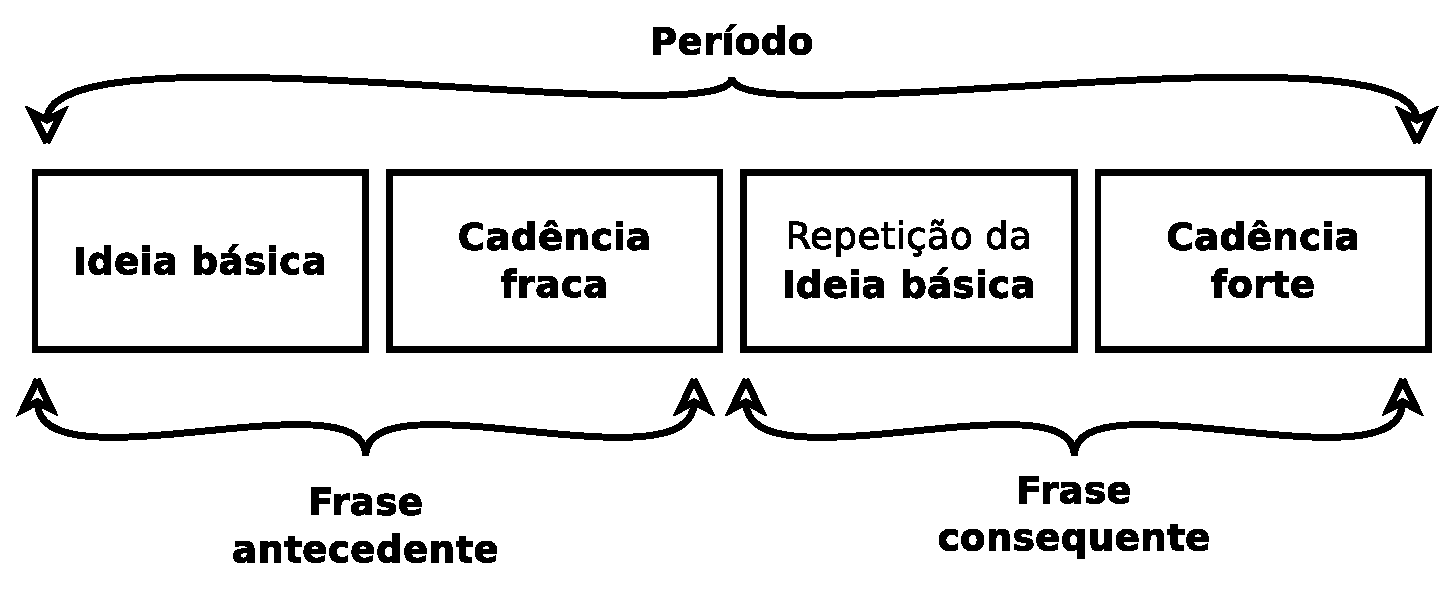
\includegraphics[width=\textwidth]{chapters/cap-musica-composer/periodo.eps}
\caption{Estrutura de uma sentença.}
\label{fig:periodostruct}
\end{figure}

\begin{example}
Na sinfonia no. 9 de Ludwig van Beethoven podemos achar exemplos do uso de períodos. 
Na Figura \ref{fig:periodo-ex1} podemos ver um período formado por 8 compassos desta sinfonia;
os 4 primeiros compassos correspondem à frase antecedente 
e os 4 últimos à frase consequente.
\end{example}

\begin{figure}[!h]
  \centering
    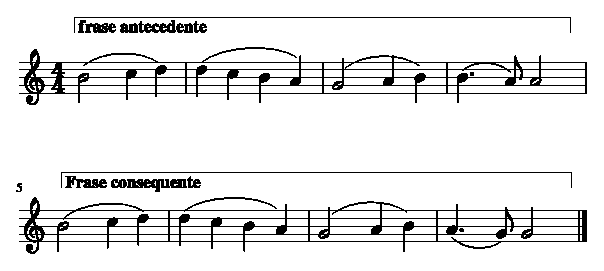
\includegraphics[width=\textwidth]{chapters/cap-musica-composer/periodo-ex1-1.eps}
\caption{Oito compassos da sinfonia no. 9, de Ludwig van Beethoven.}
\label{fig:periodo-ex1}
\end{figure}


 
\section{\textcolor{red}{Sentencia}}\index{Música!Sentencia}
% https://en.wikipedia.org/wiki/Sentence_(music)

\section{Tema}
\label{sec:tema}
\index{Música!Tema}

O tema ou também denominado sujeito (assunto) ou frase principal,
é o termo que se usa para designar aos passagens melódicos mais importantes de uma obra, 
que conservam um rasgo de continuidade \cite[pp. 411]{stainer2009dictionary} \cite[pp. 1496]{latham2008diccionario}.
Com diferença do termo \hyperref[sec:Motivo]{\textbf{motivo}},
o termo tema é usado para designar a \hyperref[sec:Frase]{\textbf{frases}} completas 
ou \hyperref[sec:Periodo]{\textbf{períodos}} \cite[pp. 1496]{latham2008diccionario},
por outro lado um motivo é muito mais curto e geralmente fragmentário \cite[pp. 545]{apel1969harvard},
para mais detalhes ir a Seção \ref{sec:Motivo}.

O tema é a frase principal de um movimento \cite[pp. 411]{stainer2009dictionary};
porem,  em movimentos em forma de sonata, 
devem existir  dois  temas principais sendo eles os primeiro e o segundo no movimento, e
tem o maior peso estrutural da mesma \cite[pp. 411]{stainer2009dictionary} \cite[pp. 1496]{latham2008diccionario}.

Existem composições politemáticas e monotemáticas;
é dizer com vários temas ou um tema, respectivamente; 
como já vimos, entre os exemplos de composições politemáticas,
temos as sonatas; e como exemplo para composições monotemáticas temos as fugas \cite[pp. 539]{apel1969harvard}.

\begin{example}
Na cultura moderna atual, os temas podem ser mais facilmente reconhecidos  na música cinematográfica.
Por exemplo, para muitos de nós, ficaram marcados os temas dos filmes: ``Superman'', ``Indiana Jones'',
``Star Wars'', ``O grande chefão (The Godfather)'', ``Harry Potter'', etc.
Em algumas ocasiões, os temas podem corresponder aos protagonistas, 
e em outros casos os temas podem fazer referencia a algum elemento na trama.
Porem em todos os casos estão bem gravados na nossa mente, 
de modo que ao escutá-los nos sentimos irreversivelmente obrigados a lembrar seu filme de origem.
\end{example}
  
%\section{\textcolor{red}{Riff}}\index{Música!Riff}
% https://es.wikipedia.org/wiki/Riff
\cite[pp. 1440,1477]{latham2008diccionario}
 




\section{A forma musical}
\label{sec:FormaMusical}
\index{Música!Forma musical}

\begin{tcbinformation} 
\textbf{Seção:}
\index{Música!Seção}
\label{ref:Secao}
No sentido mais amplo, uma seção é uma divisão curta de uma composição;
sendo as seções limitadas rítmica e harmonicamente para ser entes diferenciados \cite[pp. 174]{baker1895dictionary}.
As seções geralmente tem forma de frases, períodos, sentenças, etc. 
\end{tcbinformation} 

A ``forma'' musical é o jeito em que os compositores organizam as \hyperref[ref:Secao]{\textbf{seções}} numa peça musical.
Cada seção se representa mediante uma letra maiúscula (ex: $A$, $B$, $C$, $D$, etc.) \cite[pp. 71]{bennett1993elementos};
assim, escrever $ABCBA$, indica que a peça musical tem as seções $A$, $B$ e $C$,
e que são executadas seguindo a ordem $A$, $B$, $C$, $B$ e finalmente $A$.


Os compositores utilizam sobre as seções os seguintes princípios estruturais:
\begin{description}
\item[Repetição:] Se refere a repetição das seções (ex: $AAA...A$) 
\cite[pp. 71]{bennett1993elementos} \cite[pp. 88]{howard1991aprendendo} \cite[pp. 53]{colluraimprovisacao} 
\cite[pp. 85]{holland2013music}.
A repetição é relativa à altura das notas, 
pois a letra que acompanha pode variar drasticamente entre seções.
 
\item[Variação :] Indica a repetição com variação das seções, 
 com o fim de manter o interesse na música
\cite[pp. 71]{bennett1993elementos} \cite[pp. 88]{howard1991aprendendo} \cite[pp. 53]{colluraimprovisacao}.
Geralmente se indica com $A'$ a variação de A (ex: $AA'A''$).

\item[Contraste:] O contraste é outro jeito de manter o interesse do 
público, onde as seções são  marcadamente diferenciadas e com ideias novas
\cite[pp. 71]{bennett1993elementos} \cite[pp. 88]{howard1991aprendendo} 
\cite[pp. 53]{colluraimprovisacao}  \cite[pp. 85]{holland2013music}.
Se $A$ é uma seção que contrasta com $B$, poderíamos escrever: $AB$, ou $ABA$.
\begin{example}
Se a estrofe é $A$ e o coro é $B$ então:
\begin{itemize} 
\item estrofe: caráter tranquilo, registro grave, um cantante, acordes menores, etc.
\item coro: caráter enérgico, registro agudo, vários cantantes, acordes maiores, etc.
\end{itemize}
\end{example}
\end{description} 

Entre as formas mais conhecidas de estruturar as seções, temos:
A \hyperref[subsec:formabinaria]{\textbf{forma binária}}, 
a \hyperref[subsec:formaternaria]{\textbf{forma ternária}}, 
a \hyperref[subsec:formarondo]{\textbf{forma rondó}}, 
a \hyperref[subsec:formacancao]{\textbf{forma canção}}, 
a \hyperref[subsec:formaabac]{\textbf{forma $\mathbf{ABAC}$}}, 
etc.
 



\subsection{Forma binária: $AB$}
\label{subsec:formabinaria}
\index{Música!Forma binária}
Uma peça musical em forma binária está constituída por duas seções 
com um peso equivalente; 
a estas seções as designaremos com as letras $A$ e $B$, 
onde $B$ pode ser maior ou igual que $A$ em duração; juntos
formam a estrutura $AB$;
ambas seções pode ter sinal de repetição; se é assim, então é possivel ver estruturas como 
\cite[pp. 71]{bennett1993elementos} \cite[pp. 93]{copland1974ouvir}:
\begin{itemize}
\item $AB$,
\item $AAB$ (é dizer $||:A:||B$) ou 
\item $AABB$ (é dizer $||:A:||:B:||$).
\end{itemize}
Depois das partes A e B, 
pode haver uma \hyperref[ref:Coda]{\textbf{coda}} 
ou uma seção final mais longa \cite[pp. 86-87]{holland2013music}.

\begin{example} ~
\begin{itemize}
\item ``Mamãe eu quero'' de Vicente Paiva e Jararaca,
interpretado por Carmen Miranda no filme ``Down Argentine Way'' de 1940. 
Tem seções de 8 compassos,
com o seguinte formato:
Introdução, $AB$, $||:A:||B$, $||:A:||^3$, final.
\end{itemize}
\end{example}




\subsection{Forma ternaria: $ABA$}
\label{subsec:formaternaria}
\index{Música!Forma ternária}
Uma peça musical em forma ternária está constituída por três seções 
estruturadas na ordem $ABA$; 
onde a seção $A$ se repete no final,
porém na segunda vez que se repete $A$,
modificações podem ser introduzidas \cite[pp. 71]{bennett1993elementos} \cite[pp. 88]{holland2013music}.


Seguindo  Aaron Copland, autor do livro ``Como ouvir e entender música'' \cite[pp. 89]{copland1974ouvir},
a forma ternaria se mantem, mesmo que seção $A$ seja repetida;
então é possivel ver estruturas como: 
\begin{itemize}
\item $ABA$ ou
\item $AABA$ (é dizer $||:A:||BA$).
\end{itemize}

\begin{example} ~
\begin{itemize}
\item ``Garota de Ipanema'' de Antônio Carlos Jobim e interpretado por Gal Costa,
com a seções de 8 compassos binários \cite{partituragarotaipanema1} \cite{partituragarotaipanema2}.
Tem uma estrutura: Introdução, $||:A:||:B:||A$, solo,  $||:A:||:B:||A$, final.
Com a introdução, e final de 8 compassos binários, 
e um solo com 5 seçoes de 8 compassos binários.
\end{itemize}
\end{example}

\subsubsection{Forma canção: $AABA$}
\label{subsec:formacancao}
\index{Música!Forma canção}
Uma peça musical em forma canção está constituída por duas seções, $A$ e $B$,
seguindo uma estrutura $AABA$; 
onde a seção $A$ se repete sempre variando um pouco suas carateristicas;
é comum ver seções de 8 compassos de duração, mas podem existir casos diferentes
\cite[pp. 53]{colluraimprovisacao} \cite[pp. 16]{adolfo1997composicao}.
\begin{example} ~
\begin{itemize}
\item ``Samba de uma nota só'' de Antônio Carlos Jobim \cite[pp. 53]{colluraimprovisacao} \cite[pp. 16]{adolfo1997composicao},
com seções de 8 compassos binários \cite{partiturasambadeumanotaso1}.
\end{itemize}
\end{example}

\subsection{Forma rondó: $ABACA$}
\label{subsec:formarondo}
\index{Música!Forma rondó}
Uma peça na forma rondó está composta por seções, 
chamadas aqui episódios, onde estas são rondadas pela seção inicial;
é dizer temos estruturas como $ABACA$, onde os episódios $B$ e $C$,
estão sendo rondados por $A$;
Cada vez que a seção $A$ se repete, 
pequenas modificações podem ser feitas \cite[pp. 72]{bennett1993elementos}.
Então é possivel ver estruturas como: 
\begin{itemize}
\item $ABACA$,
\item $ABACADA$ \cite[pp. 98]{copland1974ouvir},
\item $AABBACCA$ (é dizer $||:A:||:B:||A||:C:||A$).
\end{itemize}

\subsubsection{Forma $AABBACCA$: Choro}
\label{subsec:formachoro}
\index{Música!Forma do choro}
Uma peça musical na forma $AABBACCA$, é a forma típica do choro;
onde as seções $B$ e $C$ são contruidos nas regiões da dominante ou da subdominante 
\cite[pp. 83]{colluraimprovisacao}.
Esta forma é uma forma rondó escrita como  $||:A:||:B:||A||:C:||A$ \cite[pp. 53]{diniz2003almanaque}.
\begin{example} ~
\begin{itemize}
\item ``Espinha de bacalhau''  de Severino Araújo \cite[pp. 83]{colluraimprovisacao},
com seções de 16 compassos.
\item ``Cuidado, colega''  de Ernesto Nazareth \cite[pp. 83]{colluraimprovisacao},
com seções de 16 compassos.
\item ``Odeon'' de Ernesto Nazareth. Tem seções de 16 compassos binários.
\end{itemize}
\end{example}



\subsection{Forma $ABAC$}
\label{subsec:formaabac}
\index{Música!Forma $ABAC$}
Uma peça musical nesta forma está constituída por três seções, $A$, $B$ e $C$,
seguindo uma estrutura $ABAC$; 
é comum ver seções de 8 compassos de duração, mas podem existir casos diferentes
\cite[pp. 53]{colluraimprovisacao}.
\begin{example} ~
\begin{itemize}
\item ``Corcovado''  de Antônio Carlos Jobim \cite[pp. 53]{colluraimprovisacao},
com a seções de 8 compassos binários \cite{partituracorcovado1}.
\item ``Samba de verão'' de Marcos e Paulo Sérgio Valle  \cite[pp. 53]{colluraimprovisacao},
com a seções de 8 compassos quaternários.
\end{itemize}
\end{example}


%%%%%%%%%%%%%%%%%%%%%%%%%%%%%%%%%%%%%%%%%%%%%%%%%%%%%%%%%%%%%%%%%%%%%%
%\cite[pp. 289]{duckworth2007creative}
  


